%% bare_jrnl.tex
%% V1.4b
%% 2015/08/26
%% by Michael Shell
%% see http://www.michaelshell.org/
%% for current contact information.
%%
%% This is a skeleton file demonstrating the use of IEEEtran.cls
%% (requires IEEEtran.cls version 1.8b or later) with an IEEE
%% journal paper.
%%
%% Support sites:
%% http://www.michaelshell.org/tex/ieeetran/
%% http://www.ctan.org/pkg/ieeetran
%% and
%% http://www.ieee.org/ dafa Julio asdfagd lg;adsflkaj

%%*************************************************************************
%% Legal Notice:
%% This code is offered as-is without any warranty either expressed or
%% implied; without even the implied warranty of MERCHANTABILITY or
%% FITNESS FOR A PARTICULAR PURPOSE! 
%% User assumes all risk.
%% In no event shall the IEEE or any contributor to this code be liable for
%% any damages or losses, including, but not limited to, incidental,
%% consequential, or any other damages, resulting from the use or misuse
%% of any information contained here.
%%
%% All comments are the opinions of their respective authors and are not
%% necessarily endorsed by the IEEE.
%%
%% This work is distributed under the LaTeX Project Public License (LPPL)
%% ( http://www.latex-project.org/ ) version 1.3, and may be freely used,
%% distributed and modified. A copy of the LPPL, version 1.3, is included
%% in the base LaTeX documentation of all distributions of LaTeX released
%% 2003/12/01 or later.
%% Retain all contribution notices and credits.
%% ** Modified files should be clearly indicated as such, including  **
%% ** renaming them and changing author support contact information. **
%%*************************************************************************


% *** Authors should verify (and, if needed, correct) their LaTeX system  ***
% *** with the testflow diagnostic prior to trusting their LaTeX platform ***
% *** with production work. The IEEE's font choices and paper sizes can   ***
% *** trigger bugs that do not appear when using other class files.       ***                          ***
% The testflow support page is at:
% http://www.michaelshell.org/tex/testflow/



\documentclass[journal]{IEEEtran}
%
% If IEEEtran.cls has not been installed into the LaTeX system files,
% manually specify the path to it like:
% \documentclass[journal]{../sty/IEEEtran}





% Some very useful LaTeX packages include:
% (uncomment the ones you want to load)


% *** MISC UTILITY PACKAGES ***
%
%\usepackage{ifpdf}
% Heiko Oberdiek's ifpdf.sty is very useful if you need conditional
% compilation based on whether the output is pdf or dvi.
% usage:
% \ifpdf
%   % pdf code
% \else
%   % dvi code
% \fi
% The latest version of ifpdf.sty can be obtained from:
% http://www.ctan.org/pkg/ifpdf
% Also, note that IEEEtran.cls V1.7 and later provides a builtin
% \ifCLASSINFOpdf conditional that works the same way.
% When switching from latex to pdflatex and vice-versa, the compiler may
% have to be run twice to clear warning/error messages.






% *** CITATION PACKAGES ***
%
%\usepackage{cite}
% cite.sty was written by Donald Arseneau
% V1.6 and later of IEEEtran pre-defines the format of the cite.sty package
% \cite{} output to follow that of the IEEE. Loading the cite package will
% result in citation numbers being automatically sorted and properly
% "compressed/ranged". e.g., [1], [9], [2], [7], [5], [6] without using
% cite.sty will become [1], [2], [5]--[7], [9] using cite.sty. cite.sty's
% \cite will automatically add leading space, if needed. Use cite.sty's
% noadjust option (cite.sty V3.8 and later) if you want to turn this off
% such as if a citation ever needs to be enclosed in parenthesis.
% cite.sty is already installed on most LaTeX systems. Be sure and use
% version 5.0 (2009-03-20) and later if using hyperref.sty.
% The latest version can be obtained at:
% http://www.ctan.org/pkg/cite
% The documentation is contained in the cite.sty file itself.






% *** GRAPHICS RELATED PACKAGES ***
%
\ifCLASSINFOpdf
  % \usepackage[pdftex]{graphicx}
  % declare the path(s) where your graphic files are
  % \graphicspath{{../pdf/}{../jpeg/}}
  % and their extensions so you won't have to specify these with
  % every instance of \includegraphics
  % \DeclareGraphicsExtensions{.pdf,.jpeg,.png}
\else
  % or other class option (dvipsone, dvipdf, if not using dvips). graphicx
  % will default to the driver specified in the system graphics.cfg if no
  % driver is specified.
  % \usepackage[dvips]{graphicx}
  % declare the path(s) where your graphic files are
  % \graphicspath{{../eps/}}
  % and their extensions so you won't have to specify these with
  % every instance of \includegraphics
  % \DeclareGraphicsExtensions{.eps}
\fi
% graphicx was written by David Carlisle and Sebastian Rahtz. It is
% required if you want graphics, photos, etc. graphicx.sty is already
% installed on most LaTeX systems. The latest version and documentation
% can be obtained at: 
% http://www.ctan.org/pkg/graphicx
% Another good source of documentation is "Using Imported Graphics in
% LaTeX2e" by Keith Reckdahl which can be found at:
% http://www.ctan.org/pkg/epslatex
%
% latex, and pdflatex in dvi mode, support graphics in encapsulated
% postscript (.eps) format. pdflatex in pdf mode supports graphics
% in .pdf, .jpeg, .png and .mps (metapost) formats. Users should ensure
% that all non-photo figures use a vector format (.eps, .pdf, .mps) and
% not a bitmapped formats (.jpeg, .png). The IEEE frowns on bitmapped formats
% which can result in "jaggedy"/blurry rendering of lines and letters as
% well as large increases in file sizes.
%
% You can find documentation about the pdfTeX application at:
% http://www.tug.org/applications/pdftex





% *** MATH PACKAGES ***
%
%\usepackage{amsmath}
% A popular package from the American Mathematical Society that provides
% many useful and powerful commands for dealing with mathematics.
%
% Note that the amsmath package sets \interdisplaylinepenalty to 10000
% thus preventing page breaks from occurring within multiline equations. Use:
%\interdisplaylinepenalty=2500
% after loading amsmath to restore such page breaks as IEEEtran.cls normally
% does. amsmath.sty is already installed on most LaTeX systems. The latest
% version and documentation can be obtained at:
% http://www.ctan.org/pkg/amsmath





% *** SPECIALIZED LIST PACKAGES ***
%
%\usepackage{algorithmic}
% algorithmic.sty was written by Peter Williams and Rogerio Brito.
% This package provides an algorithmic environment fo describing algorithms.
% You can use the algorithmic environment in-text or within a figure
% environment to provide for a floating algorithm. Do NOT use the algorithm
% floating environment provided by algorithm.sty (by the same authors) or
% algorithm2e.sty (by Christophe Fiorio) as the IEEE does not use dedicated
% algorithm float types and packages that provide these will not provide
% correct IEEE style captions. The latest version and documentation of
% algorithmic.sty can be obtained at:
% http://www.ctan.org/pkg/algorithms
% Also of interest may be the (relatively newer and more customizable)
% algorithmicx.sty package by Szasz Janos:
% http://www.ctan.org/pkg/algorithmicx




% *** ALIGNMENT PACKAGES ***
%
%\usepackage{array}
% Frank Mittelbach's and David Carlisle's array.sty patches and improves
% the standard LaTeX2e array and tabular environments to provide better
% appearance and additional user controls. As the default LaTeX2e table
% generation code is lacking to the point of almost being broken with
% respect to the quality of the end results, all users are strongly
% advised to use an enhanced (at the very least that provided by array.sty)
% set of table tools. array.sty is already installed on most systems. The
% latest version and documentation can be obtained at:
% http://www.ctan.org/pkg/array


% IEEEtran contains the IEEEeqnarray family of commands that can be used to
% generate multiline equations as well as matrices, tables, etc., of high
% quality.




% *** SUBFIGURE PACKAGES ***
%\ifCLASSOPTIONcompsoc
%  \usepackage[caption=false,font=normalsize,labelfont=sf,textfont=sf]{subfig}
%\else
%  \usepackage[caption=false,font=footnotesize]{subfig}
%\fi
% subfig.sty, written by Steven Douglas Cochran, is the modern replacement
% for subfigure.sty, the latter of which is no longer maintained and is
% incompatible with some LaTeX packages including fixltx2e. However,
% subfig.sty requires and automatically loads Axel Sommerfeldt's caption.sty
% which will override IEEEtran.cls' handling of captions and this will result
% in non-IEEE style figure/table captions. To prevent this problem, be sure
% and invoke subfig.sty's "caption=false" package option (available since
% subfig.sty version 1.3, 2005/06/28) as this is will preserve IEEEtran.cls
% handling of captions.
% Note that the Computer Society format requires a larger sans serif font
% than the serif footnote size font used in traditional IEEE formatting
% and thus the need to invoke different subfig.sty package options depending
% on whether compsoc mode has been enabled.
%
% The latest version and documentation of subfig.sty can be obtained at:
% http://www.ctan.org/pkg/subfig




% *** FLOAT PACKAGES ***
%
%\usepackage{fixltx2e}
% fixltx2e, the successor to the earlier fix2col.sty, was written by
% Frank Mittelbach and David Carlisle. This package corrects a few problems
% in the LaTeX2e kernel, the most notable of which is that in current
% LaTeX2e releases, the ordering of single and double column floats is not
% guaranteed to be preserved. Thus, an unpatched LaTeX2e can allow a
% single column figure to be placed prior to an earlier double column
% figure.
% Be aware that LaTeX2e kernels dated 2015 and later have fixltx2e.sty's
% corrections already built into the system in which case a warning will
% be issued if an attempt is made to load fixltx2e.sty as it is no longer
% needed.
% The latest version and documentation can be found at:
% http://www.ctan.org/pkg/fixltx2e


%\usepackage{stfloats}
% stfloats.sty was written by Sigitas Tolusis. This package gives LaTeX2e
% the ability to do double column floats at the bottom of the page as well
% as the top. (e.g., "\begin{figure*}[!b]" is not normally possible in
% LaTeX2e). It also provides a command:
%\fnbelowfloat
% to enable the placement of footnotes below bottom floats (the standard
% LaTeX2e kernel puts them above bottom floats). This is an invasive package
% which rewrites many portions of the LaTeX2e float routines. It may not work
% with other packages that modify the LaTeX2e float routines. The latest
% version and documentation can be obtained at:
% http://www.ctan.org/pkg/stfloats
% Do not use the stfloats baselinefloat ability as the IEEE does not allow
% \baselineskip to stretch. Authors submitting work to the IEEE should note
% that the IEEE rarely uses double column equations and that authors should try
% to avoid such use. Do not be tempted to use the cuted.sty or midfloat.sty
% packages (also by Sigitas Tolusis) as the IEEE does not format its papers in
% such ways.
% Do not attempt to use stfloats with fixltx2e as they are incompatible.
% Instead, use Morten Hogholm'a dblfloatfix which combines the features
% of both fixltx2e and stfloats:
%
% \usepackage{dblfloatfix}
% The latest version can be found at:
% http://www.ctan.org/pkg/dblfloatfix




%\ifCLASSOPTIONcaptionsoff
%  \usepackage[nomarkers]{endfloat}
% \let\MYoriglatexcaption\caption
% \renewcommand{\caption}[2][\relax]{\MYoriglatexcaption[#2]{#2}}
%\fi
% endfloat.sty was written by James Darrell McCauley, Jeff Goldberg and 
% Axel Sommerfeldt. This package may be useful when used in conjunction with 
% IEEEtran.cls'  captionsoff option. Some IEEE journals/societies require that
% submissions have lists of figures/tables at the end of the paper and that
% figures/tables without any captions are placed on a page by themselves at
% the end of the document. If needed, the draftcls IEEEtran class option or
% \CLASSINPUTbaselinestretch interface can be used to increase the line
% spacing as well. Be sure and use the nomarkers option of endfloat to
% prevent endfloat from "marking" where the figures would have been placed
% in the text. The two hack lines of code above are a slight modification of
% that suggested by in the endfloat docs (section 8.4.1) to ensure that
% the full captions always appear in the list of figures/tables - even if
% the user used the short optional argument of \caption[]{}.
% IEEE papers do not typically make use of \caption[]'s optional argument,
% so this should not be an issue. A similar trick can be used to disable
% captions of packages such as subfig.sty that lack options to turn off
% the subcaptions:
% For subfig.sty:
% \let\MYorigsubfloat\subfloat
% \renewcommand{\subfloat}[2][\relax]{\MYorigsubfloat[]{#2}}
% However, the above trick will not work if both optional arguments of
% the \subfloat command are used. Furthermore, there needs to be a
% description of each subfigure *somewhere* and endfloat does not add
% subfigure captions to its list of figures. Thus, the best approach is to
% avoid the use of subfigure captions (many IEEE journals avoid them anyway)
% and instead reference/explain all the subfigures within the main caption.
% The latest version of endfloat.sty and its documentation can obtained at:
% http://www.ctan.org/pkg/endfloat
%
% The IEEEtran \ifCLASSOPTIONcaptionsoff conditional can also be used
% later in the document, say, to conditionally put the References on a 
% page by themselves.




% *** PDF, URL AND HYPERLINK PACKAGES ***
%
%\usepackage{url}
% url.sty was written by Donald Arseneau. It provides better support for
% handling and breaking URLs. url.sty is already installed on most LaTeX
% systems. The latest version and documentation can be obtained at:
% http://www.ctan.org/pkg/url
% Basically, \url{my_url_here}.




% *** Do not adjust lengths that control margins, column widths, etc. ***
% *** Do not use packages that alter fonts (such as pslatex).         ***
% There should be no need to do such things with IEEEtran.cls V1.6 and later.
% (Unless specifically asked to do so by the journal or conference you plan
% to submit to, of course. )


% correct bad hyphenation here
\hyphenation{op-tical net-works semi-conduc-tor}

\usepackage{graphicx}
\usepackage{float}
\usepackage{subcaption}
\usepackage{booktabs}
\begin{document}
%
% paper title
% Titles are generally capitalized except for words such as a, an, and, as,
% at, but, by, for, in, nor, of, on, or, the, to and up, which are usually
% not capitalized unless they are the first or last word of the title.
% Linebreaks \\ can be used within to get better formatting as desired.
% Do not put math or special symbols in the title.
\title{Implementation of an open-source design Flow for nano scale Chip Design/Manufacturing Process at Universidad del valle de Guatemala }
%
%
% author names and IEEE memberships
% note positions of commas and nonbreaking spaces ( ~ ) LaTeX will not break
% a structure at a ~ so this keeps an author's name from being broken across
% two lines.
% use \thanks{} to gain access to the first footnote area
% a separate \thanks must be used for each paragraph as LaTeX2e's \thanks
% was not built to handle multiple paragraphs
%

\author{Angel~Orellana,~\IEEEmembership{Member,~UVG,}
        Julio~Lopez,~\IEEEmembership{Member,~UVG,}
        Noel~Prado,~\IEEEmembership{Member,~UVG,}
        and~Daniel~Mundo,~\IEEEmembership{Member,~UVG}% <-this % stops a space
\thanks{M. Shell was with the Department
of Electrical and Computer Engineering, Georgia Institute of Technology, Atlanta,
GA, 30332 USA e-mail: (see http://www.michaelshell.org/contact.html).}% <-this % stops a space
\thanks{J. Doe and J. Doe are with Anonymous University.}% <-this % stops a space
\thanks{Manuscript received April 19, 2005; revised August 26, 2015.}}

% note the % following the last \IEEEmembership and also \thanks - 
% these prevent an unwanted space from occurring between the last author name
% and the end of the author line. i.e., if you had this:
% 
% \author{....lastname \thanks{...} \thanks{...} }
%                     ^------------^------------^----Do not want these spaces!
%
% a space would be appended to the last name and could cause every name on that
% line to be shifted left slightly. This is one of those "LaTeX things". For
% instance, "\textbf{A} \textbf{B}" will typeset as "A B" not "AB". To get
% "AB" then you have to do: "\textbf{A}\textbf{B}"
% \thanks is no different in this regard, so shield the last } of each \thanks
% that ends a line with a % and do not let a space in before the next \thanks.
% Spaces after \IEEEmembership other than the last one are OK (and needed) as
% you are supposed to have spaces between the names. For what it is worth,
% this is a minor point as most people would not even notice if the said evil
% space somehow managed to creep in.



% The paper headers
\markboth{Journal of \LaTeX\ Class Files,~Vol.~14, No.~8, August~2015}%
{Shell \MakeLowercase{\textit{et al.}}: implementation an open-source design Flow for nano scale Chip Design/Manufacturing Process at Universidad del valle de Guatemala }
% The only time the second header will appear is for the odd numbered pages
% after the title page when using the twoside option.
% 
% *** Note that you probably will NOT want to include the author's ***
% *** name in the headers of peer review papers.                   ***
% You can use \ifCLASSOPTIONpeerreview for conditional compilation here if
% you desire.




% If you want to put a publisher's ID mark on the page you can do it like
% this:
%\IEEEpubid{0000--0000/00\$00.00~\copyright~2015 IEEE}
% Remember, if you use this you must call \IEEEpubidadjcol in the second
% column for its text to clear the IEEEpubid mark.



% use for special paper notices
%\IEEEspecialpapernotice{(Invited Paper)}




% make the title area
\maketitle

% As a general rule, do not put math, special symbols or citations
% in the abstract or keywords.
\begin{abstract}
This paper carries out the Tiny Tapeout initiative with 4 verilog designs,
with the intention to fully utilize and comprehend this open-source design 
flow for chip design/manufacturing and to leave proper documentation for future 
students to take advantage of this new and innovative process to enter in the 
semiconductor realm.
Two students of the Electronics Engineering department at Universidad del Valle De Guatemala were 
fortunate to attend the "2023 IEEE EDS summer School R9" where the Tiny Tapeout workshop was 
held and where the first steps of this project were taken. The opportunity to learn from this 
workshop was invaluable and the knowledge gained was enough to actually carry out the 
Tiny Tapeout initiative at Universidad del Valle De Guatemala. Four designs were submitted 
on the September 5th 2023, after taking the necessary steps to get the tools and the 
design flow working. After submission the necessary verifications were made by the 
Tiny Tapeout team, on October 10th 2023 our four designs were approved for manufacturing 
and were sent to efabless for fabrication, the expected date for delivery 15th of February 2024. 
The final Tiny Tapeout 04 project had 143 submissions from 30 different countries, a total cell 
count of 82126 cells and a total area of die of 6 mm x 7.4 mm.
\end{abstract}

% Note that keywords are not normally used for peerreview papers.
\begin{IEEEkeywords}
IEEE, IEEEtran, journal, \LaTeX, paper, template.
\end{IEEEkeywords}

\IEEEpeerreviewmaketitle
\section{Introduction}
% 1st Paragraph, 
% ref [1] is:  “Semiconductor Leaders - IEEE IRDSTM.” 
The semiconductor industry -chip/microchip industry- holds a significant share in the market owing to its rapid strides in technological advancement. Over the years, there has been a noticeable trend of various companies pushing the limits of nanoscale technology, driving innovation within the sector\ \cite{IRDS2020}. This remarkable progress has been made possible primarily by two major aspects: on one hand there are  super specialised chip manufacturing hardware, that bring to life the digital representation of the chip. On the other hand there are very specialised software tools that are made by very specific software developing companies, who are responsible for making said digital representation of the chip. 

% 2st Paragraph, 
% ref [7] is: Week In Review: Semiconductor Manufacturing, Test
% ref [8] is: Intel is spending $20 billion to build two new chip plants in Arizona
Intel, Apple, AMD, Samsung and similar semiconductor industry giants have the financial resources to invest in these specialised tools and software, which are often costly due to their advanced capabilities and precision engineering [7-8]. These tools facilitate tasks such as layout design, simulation, verification, and manufacturing of semiconductor chips. By utilising such tools, these companies can explore innovative concepts, test them in virtual as well as physical environments, and fine-tune their designs before misproduction.

% 3st Paragraph, 
% ref [10] is: Design for Manufacturing Overview.
% ref [11] is: Synopsys, Cadence, Google And NVIDIA All Agree: Use AI To Help Design Chips,
% ref [12] is: What is Electronic Design Automation (EDA)? – How it Works | Synopsys.
Additionally, software development companies like Synopsys, Cadence, and Mentor Graphics play a crucial role in shaping the semiconductor landscape [11]. They continuously develop and refine software that cater to the intricate needs of chip designers and manufacturers [12]. These tools streamline workflows, improve design accuracy, and optimise manufacturing processes, ultimately leading to the production of high-quality chips that power a wide array of electronic devices, from smartphones, laptops, autonomous vehicles to sophisticated industrial equipment, all the way to life-critical biomedical equipment, satellites, and space shuttles [10]. 

% 4st Paragraph, 
% ref [13] is: Reshoring Semiconductor Manufacturing: Addressing the Workforce Challenge
% ref [15] is: A Vision and Strategy for the NSTC.
However, it's worth acknowledging that while the semiconductor industry thrives on innovation, learning about the intricacies of integrated circuit design and manufacturing processes can be very difficult [13,15]. This challenge is one of the key hurdles that stems from the gap in access to chip design and manufacturing processes between industry and academia. The tools and resources used by technology giants already mentioned are often proprietary and come with substantial financial barriers. This fination challenge creates a division between the cutting-edge practices employed in the industry and the educational resources available in academic settings\ \cite*{CSIS2023Reshoring}.

% 5st Paragraph,
Students and researchers in academia might encounter difficulties in gaining hands-on experience with the most up-to-date tools and techniques used in the semiconductor industry. Moreover, access to advanced fabrication facilities and sophisticated design software can be limited, potentially hindering their ability to fully grasp the complexities of modern chip design. The rapid pace of innovation in the industry can also make it challenging for academic curricula to keep up with the latest developments, further emphasising the disparity between theoretical knowledge and practical application.

% 6st Paragraph,
% ref [16] is: Roadmapping of Nanoelectronics for the New Electronics Industry.
% ref [19] is: Tiny Tapeout
% ref [18] is: Energizing collaborative industry-academia learning: a present case and future visions
Efforts are being made to bridge this gap by fostering collaborations between industry and academia [16]. Some companies offer educational programs, internships, and partnerships with universities, enabling students and researchers to gain exposure to state-of-the-art tools and real-world design challenges [19]. Moreover, open-source initiatives and shared research facilities aim to provide broader access to resources that were once exclusive to industry giants. By narrowing the division between industry and academia, aspiring chip designers and researchers can better prepare themselves for the demands of the semiconductor landscape [18].

% 7st Paragraph,
As the semiconductor industry propels forward with innovation, the challenge lies in ensuring that the knowledge and expertise surrounding integrated circuit design and manufacturing are accessible to all. Bridging the gap between the tools and processes utilised in industry and those available in academic settings will be crucial for nurturing the next generation of skilled professionals who can contribute to the ongoing advancements in the semiconductor field. In this work, an open-source environment for a design flow for chip manufacturing will be deployed at  Universidad del Valle de Guatemala to shorten the gap between industry and academia. 


\section{Experimental}
 In figure\ \ref{fig:ExpModelBlocks}, the main steps of this work 
 are portrayed.


 \begin{figure}[H]
    \centering
    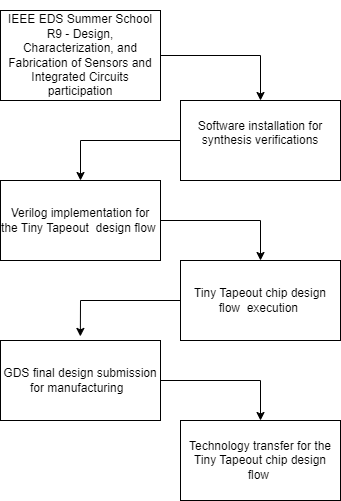
\includegraphics[width=\linewidth]{Pictures/ExperimentalModel.png}
    \caption{Experimental Model Blocks}
    \label{fig:ExpModelBlocks}
\end{figure}

\subsection{IEEE EDS Summer School R9 \- Design, Characterization, and Fabrication of Sensors and Integrated Circuits participation}
In June 2023 two senior students from the Electronics Engineering department at Universidad del Valle de Guatemala were granted scholarships 
to attend the ``2023 IEEE EDS Summer School R9" in Puebla, Mexico Throughout this enlightening summer program, a wide array of topics were 
addressed, ranging from insights of former students who work in the field, to several educational tools provided by one of the industry leaders; 
Synopsys. A significant message stood out: Nanochip design and fabrication industry is so complex, so dynamic, and so expensive due to infrastructure, 
human resources, etc. so that it becomes extremely challenging to almost impossible for academia to keep up with it.
During the program, the gap between industry capability and academic resources became evident as the alumni shared their experiences. 
Some of the former students highlighted that they had encountered setbacks in their projects due to challenges in installation or upkeep of some 
tools within the expansive realm of semiconductor technology. Notably, a few even mentioned that a lack of infrastructure and limited time had led to the 
unfortunate loss of grants they had secured for their projects.In the program, there were also discussions about new open-source tools such as Wokwi, 
designed to facilitate learning about logical circuitry. The Efabless initiative was another topic, that was introduce as a private semiconductor fabrication 
company, but the one that left the most significant impact was Tiny Tapeout because it closes de gap between the complexity behind the chip design and manufacturing 
in industry and the resources, time, and knowledge typically available in academia. This tool stood out for its adoption is further supported by a multi-purpose wafer 
and the cost-effectiveness of chip production. Typically, one of the challenges in academia involves acquiring the necessary computing power to run complex design tools. 
However, Tiny Tapeout has tackled this issue by providing its own cloud computing infrastructure, effectively reducing the demand for high computational resources. On 
the other hand, the installation of some of the highly advanced programs use in the industry are very complex using authentication servers to secure their tools, 
however Tiny Tapeout has manage to set their installation tool process very straightforward using only three steps. It’s worth mentioning that Tiny Tapeout has its 
own website where you can consult any doubt its installer might have, and it has several channels of communication. The aim of the Tiny Tapeout initiative is not 
to take over the semiconductor industry but to give students the knowledge and experience of working in this ample field, moreover, offer students the experience of taking a digital design all the way to semiconductor fabrication.


\subsection{Software installation for synthesis verifications}

To verify that both logical and physical synthesis align with the Verilog files, the installation of an  open-source integrated circuit design flow called OpenLane was performed. To use it, a virtual machine with Ubuntu 22 was set up, and the necessary prerequisites, including Python 3, git, make, and Docker, were installed. The GitHub repository containing OpenLane was cloned and compiled. It was confirmed that OpenLane operated correctly by synthesizing a 4-bit adder.
 

\subsection{Verilog implementation for the Tiny Tapeout design flow}
% Daniel 
This section introduces the Verilog implementation within the framework of Tiny Tapeout, a project dedicated to generating chip layouts from Verilog files. In this context, we will delineate the four distinct designs produced, providing comprehensive descriptions of the modules and their respective behaviors.

\subsubsection{Multi stage path for delay measurements}
The core of the module featured an approach to creating a ring oscillator. Although it was initially intended to utilize cascaded NOT gates, it was observed that the synthesizer, under the constraints of the Tiny Tapeout design flow, may replace these gates with buffers. As a result, the oscillatory behavior was expectedly altered. Nevertheless, the module's ring oscillator function was realized through a sequence of logical operations involving AND gates and inverters, forming a feedback loop. The logical signals EN and EN\_2 served as inputs to an AND\_2 module, generating a waveform represented by W\_1. Subsequently, this waveform traversed a series of inverters (tt\_prim\_inv modules), resulting in the generation of W\_2, W\_3, and cyclically returning to W\_1. While this configuration may not conform precisely to the original design intent, it offers a valuable educational opportunity to explore gate delays and their implications in digital circuitry when compared to theoretical calculations.\\

\subsubsection{ASCII Text Printer Circuit}
A Verilog module was designed to function as a text printing system capable of displaying two distinct texts, which are selected through an external signal. The module employs an internal counter synchronized with the clock to determine the specific ASCII character displayed based on the selection signal and the counter value. The output is provided through the output pins in ASCII format.\\

\subsubsection{Implementation of the Pong game}
The Verilog code, pong\_neopixel.v, with the main module "tt\_um\_pong\_neopixel", has been 
developed with the purpose of implementing a version of the Pong game on a Neopixel pixel 
matrix. This design has been conceived as an example of an interactive and playful application 
of programmable digital hardware. The "tt\_um\_pong\_neopixel" module consists of several 
inputs and outputs intended to control the game, including player input signals, start 
signals, and outputs to manage the Neopixel matrix, along with clock and reset signals. To 
ensure the stability of the input signals, "debounce" modules have been implemented. The game 
logic includes the management of the movement of the players' paddles and the ball, as well as 
collision detection and game reset when appropriate. In addition, logic has been developed to 
generate Neopixel signals that control the display on the matrix, allowing player interaction. 
This design also incorporates counters to track the sending of data to the matrix and 
appropriately selects whether LEDs should be turned on or off based on the position of the 
ball and paddles.\\

\subsubsection{Pulse Width Modulation Generator}
The Verilog code, pwm\_generator.v, with the main module "tt\_um\_pwm", is designed to 
generate a pulse width modulation (PWM) signal controlled by buttons. The module allows the duty cycle of the PWM signal to be increased or 
decreased via buttons. To ensure a reliable reading of the buttons, debounce logic is implemented that 
generates a slow clock signal (slow\_clk\_enable).\\
\subsection{Tiny Tapeout chip design flow execution}
% Daniel 
The execution of the Tiny Tapeout chip design flow begins with a series of essential steps. First it is necessary to fork the example repository provided by the Tiny Tapeout project. Once this step is completed, enabling the repository's capability to perform actions is crucial, as it allows for the automation of subsequent processes. To ensure the project's proper execution, several key tasks must be carried out. First all Verilog files must be located in the "src" folder. Additionally, the "info.yaml" file must be filled out with relevant information, including the Verilog files that constitute the design, the main design module, the authors, a project description, and, if applicable, the clock frequency. These steps are fundamental to ensuring an effective design flow and the correct implementation of chips in Tiny Tapeout.
\subsection{GDS final design submission for manufacturing}

In the final submission phase of the GDS design for 
manufacturing, a series of crucial steps were undertaken to ensure the
integrity and accuracy of the delivered information. First a comprehensive 
review of all relevant repositories was conducted with the aim of identifying
and rectifying any errors that may have existed in their execution. Subsequently
the provided form by Latin Practice was completed, requiring essential 
details about the repositories, including author names and direct links 
to the referred repositories. It is noteworthy that this form-filling 
process was rigorously carried out before the stipulated deadline, which 
was September 5th. These steps were taken to ensure the consistency and 
precision of the information provided in this critical stage of the GDS 
design project. In figures\ \ref*{fig:pwm_verified},\ \ref*{fig:pong_verified},
\ \ref*{fig:ascii_verified}, and\ \ref*{fig:delay_verified} the verification 
process of the four design sent to manufacture is shown to be successful.

\begin{figure}[tbh]
    \centering
    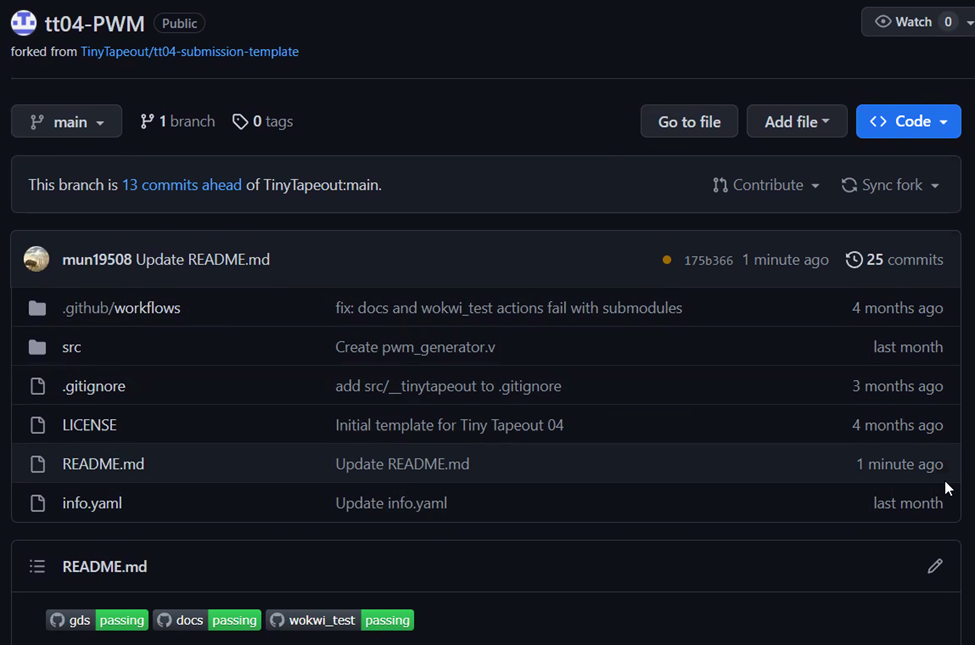
\includegraphics[width=\linewidth]{Pictures/pwm_verified.png}
    \caption{Verified Pulse Width Modulation Generator Verilog }\label{fig:pwm_verified}
\end{figure}

\begin{figure}[tbh]
    \centering
    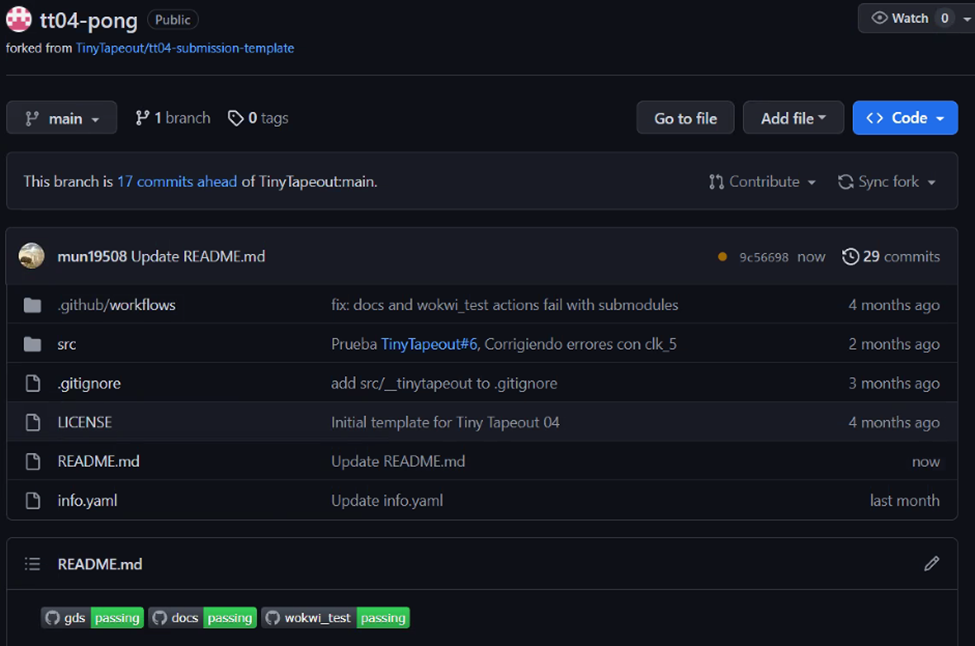
\includegraphics[width=\linewidth]{Pictures/pong.png}
    \caption{Verified Pong game Verilog}\label{fig:pong_verified}
\end{figure}

\begin{figure}[tbh]
    \centering
    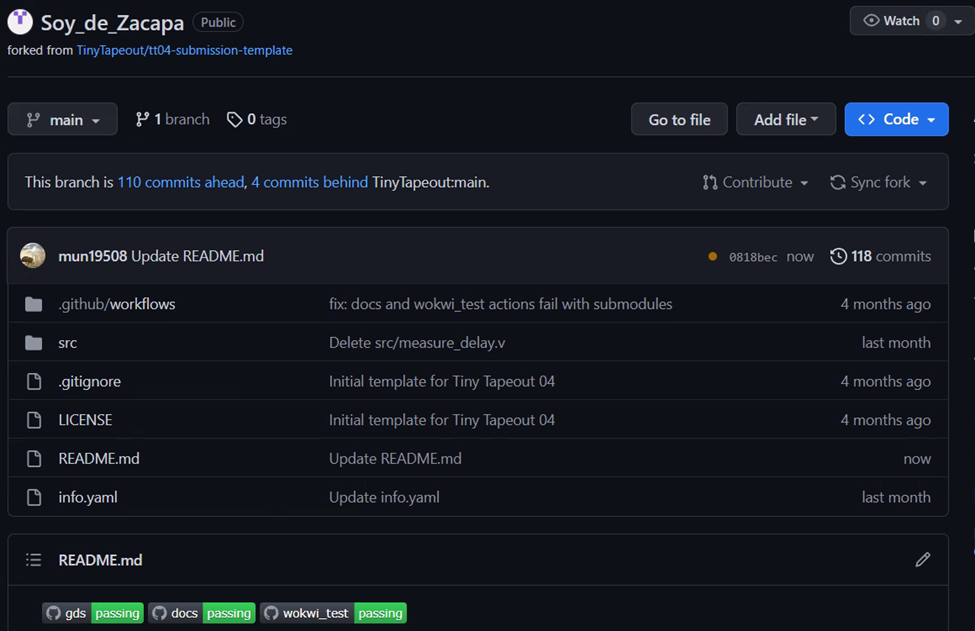
\includegraphics[width=\linewidth]{Pictures/verifide_zacapa.png}
    \caption{Verified ASCII Text Printer Circuit Verilog}\label{fig:ascii_verified}
\end{figure}

\begin{figure}[H] 
    \centering
    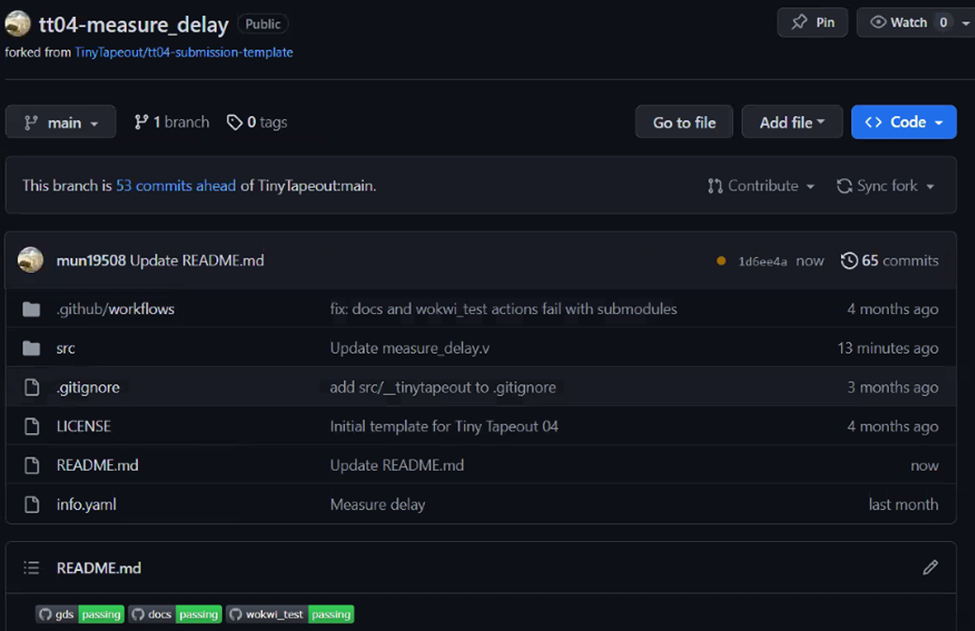
\includegraphics[width=\linewidth]{Pictures/delay_ver.png}
    \caption{Verified Multi stage path for delay measurements Verilog}\label{fig:delay_verified}
\end{figure}

\subsection{Technology transfer for the Tiny Tapeout chip design flow}

The true purpose behind this paper is to push the boundaries of understanding the semiconductor fabrication field at Universidad del Valle de Guatemala. The proper documentation of the knowledge acquired by all the members that were involved on this work is essential for future students. Therefore, Video tutorials and documents were made for students to replicate the Tiny tapeout program to take any design from a fully digital verilog implemented circuit all the way to a physical integrated circuit. 

% needed in second column of first page if using \IEEEpubid
%\IEEEpubidadjcol

\section{Results}
Following the submission of the verilog designs on September 5th, 2023, the Tiny Tapeout team began the process of verification. 
The verification process consisted of a series of proprietary tests to ensure that the designs were correct and that they would be able to be fabricated.
Subsequently, the Tiny Tapeout team reached out to confirm the approval for fabrication. The expected delivery date for the fabricated chips is on February 15th, 2024.

The use of Github has allowed the design submission process to become more automated and streamlined. The use of Github has also allowed the Tiny Tapeout team to develop 
interesting and innovative tools to aid in the intricacies of the designs making process. One of these tools is a 2D viewer that allows the user to view the final 
layout of the design on the die and a 3D viewer that allows the user to see the different layers of the design to further understand the complexity of what is behind the 
fabrication of a chip. The 2D and 3D views of each of the design submitted are shown in the figures \ref*{fig:delay_Layout}, \ref*{fig:ASCII_Layout}, \ref*{fig:Pong_Layout} and \ref*{fig:PWM} 
were generated on the git repository of the respective git projects for each of the designs.

\begin{figure}[H]
    \centering
    \begin{subfigure}[b]{0.45\textwidth}
        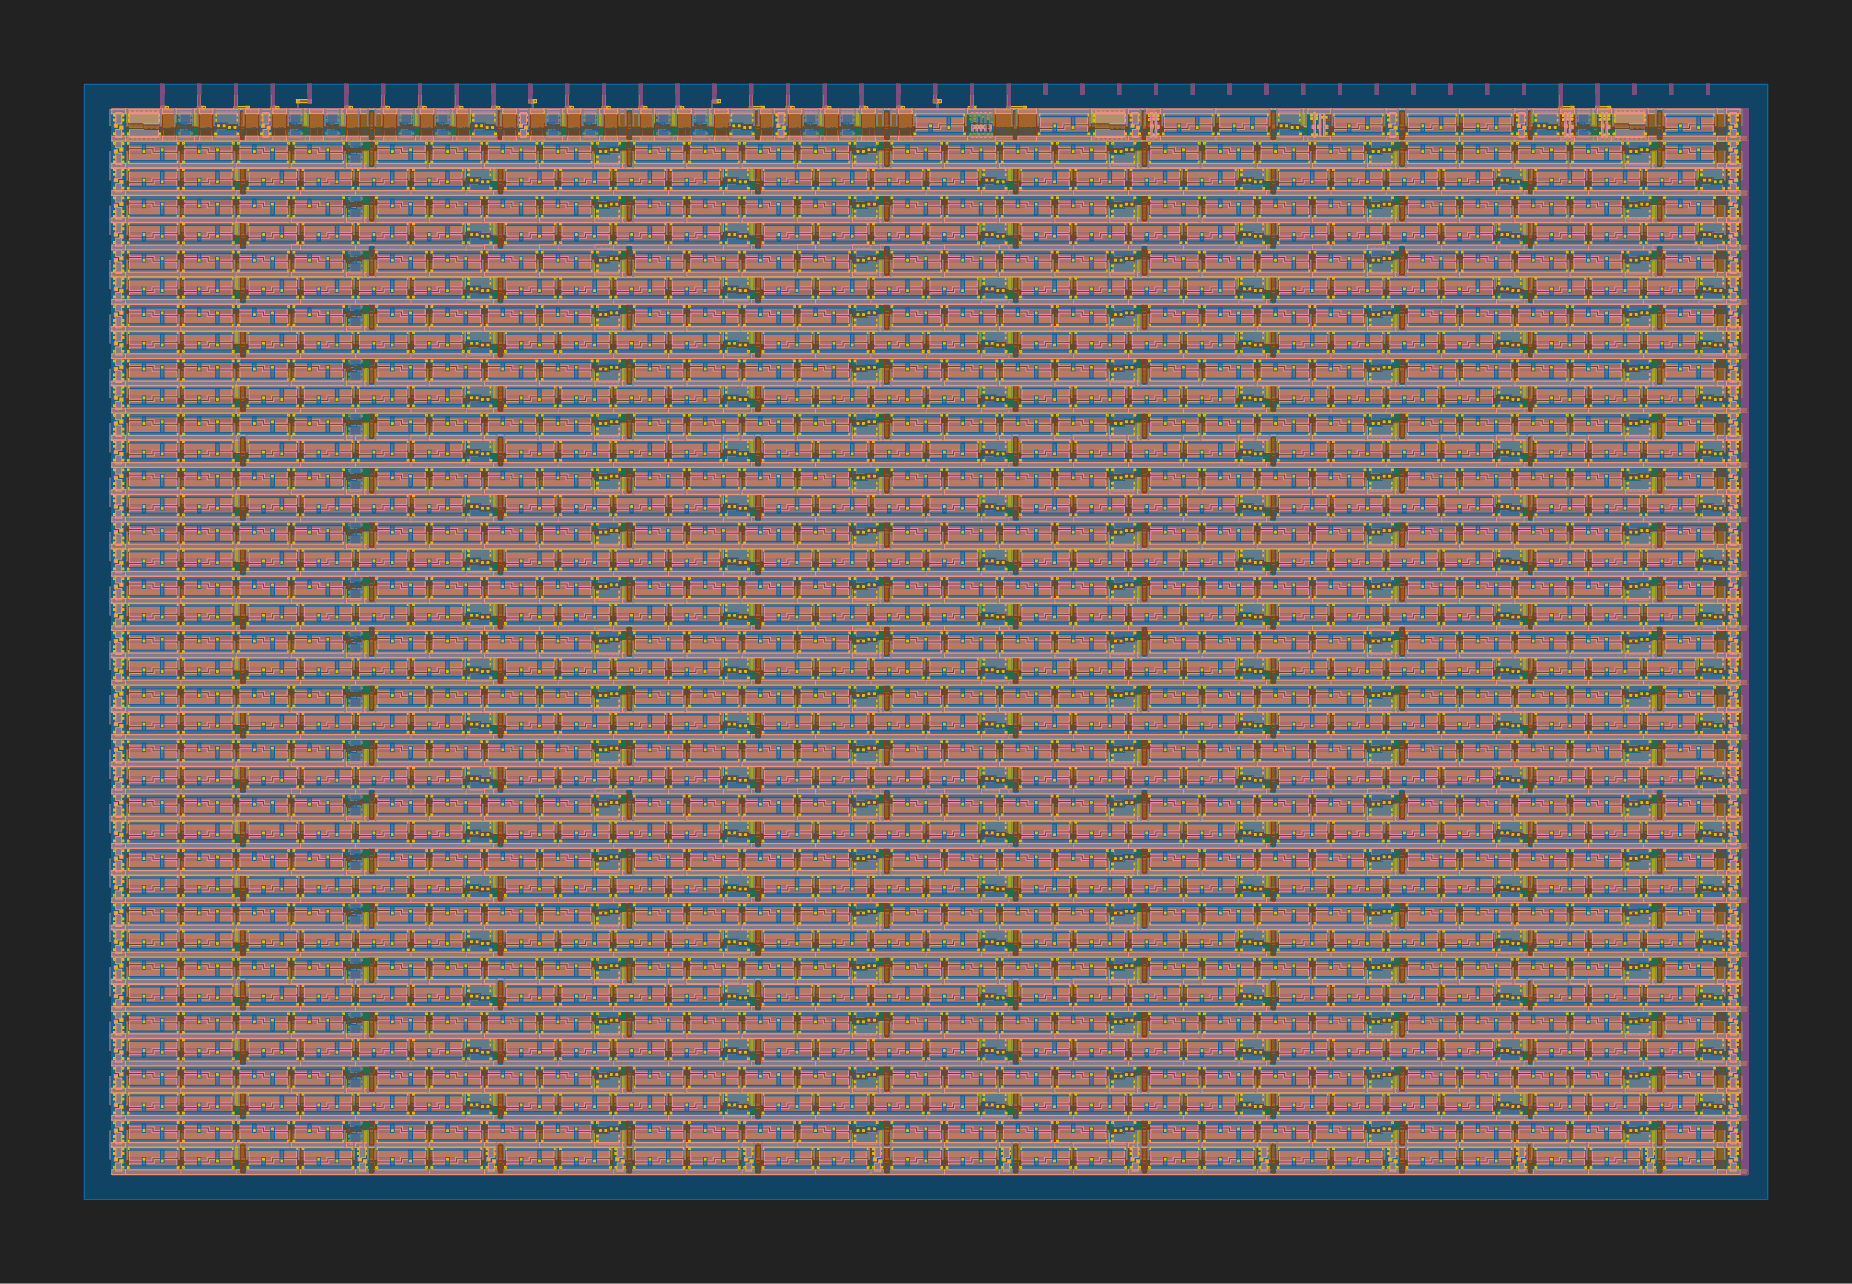
\includegraphics[width=\linewidth]{Pictures/Result_Delay_2D_View.png}
        \caption{View 2D}\label{fig:delay_2D}
    \end{subfigure}
    \begin{subfigure}[b]{0.45\textwidth}
        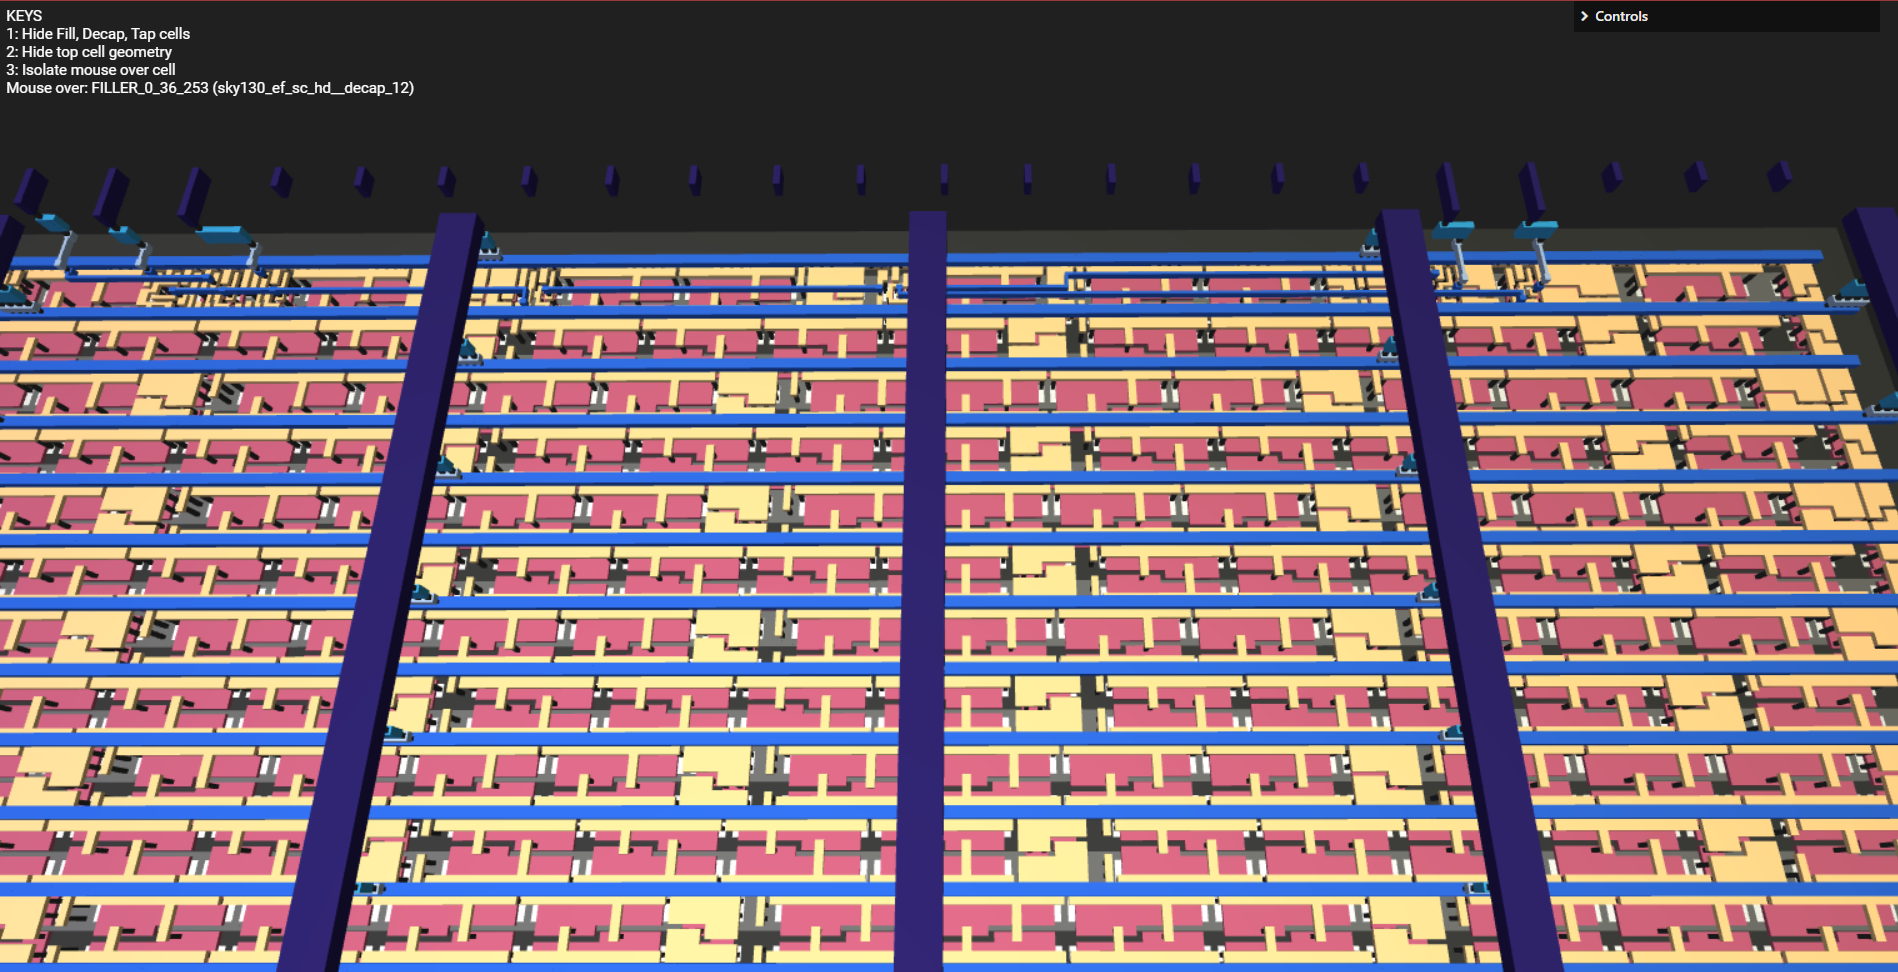
\includegraphics[width=\linewidth]{Pictures/Result_Delay_3D_View.png}
        \caption{View 3D}\label{fig:delay_3D}
    \end{subfigure}
    \caption{multistage path for delay measurements layout}\label{fig:delay_Layout}
\end{figure}

\begin{figure}[H]
    \centering
    \begin{subfigure}[b]{0.45\textwidth}
        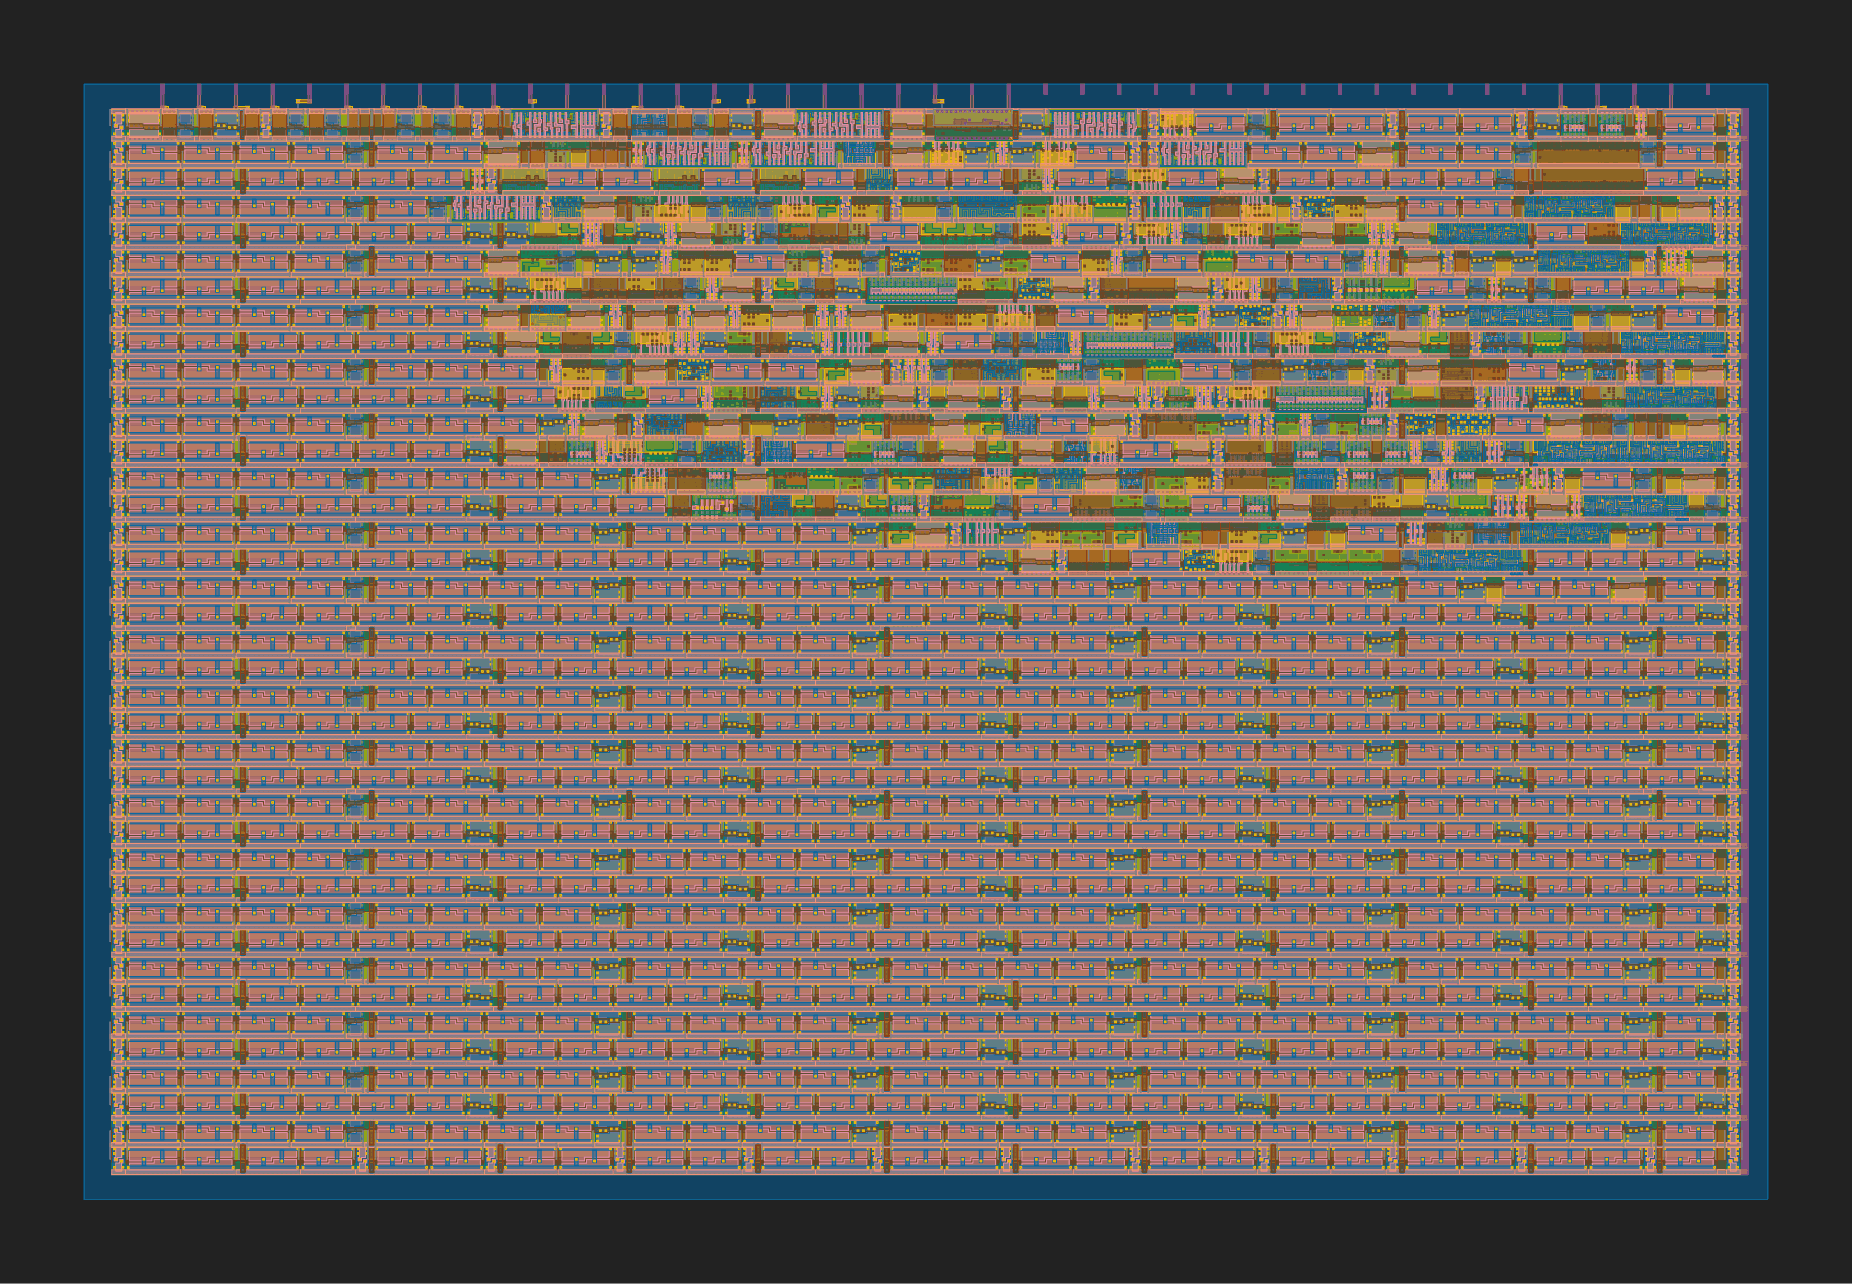
\includegraphics[width=\linewidth]{Pictures/Result_ASCII_2D_View.png}
        \caption{View 2D}\label{fig:ASCII_2D}
    \end{subfigure}
    \begin{subfigure}[b]{0.45\textwidth}
        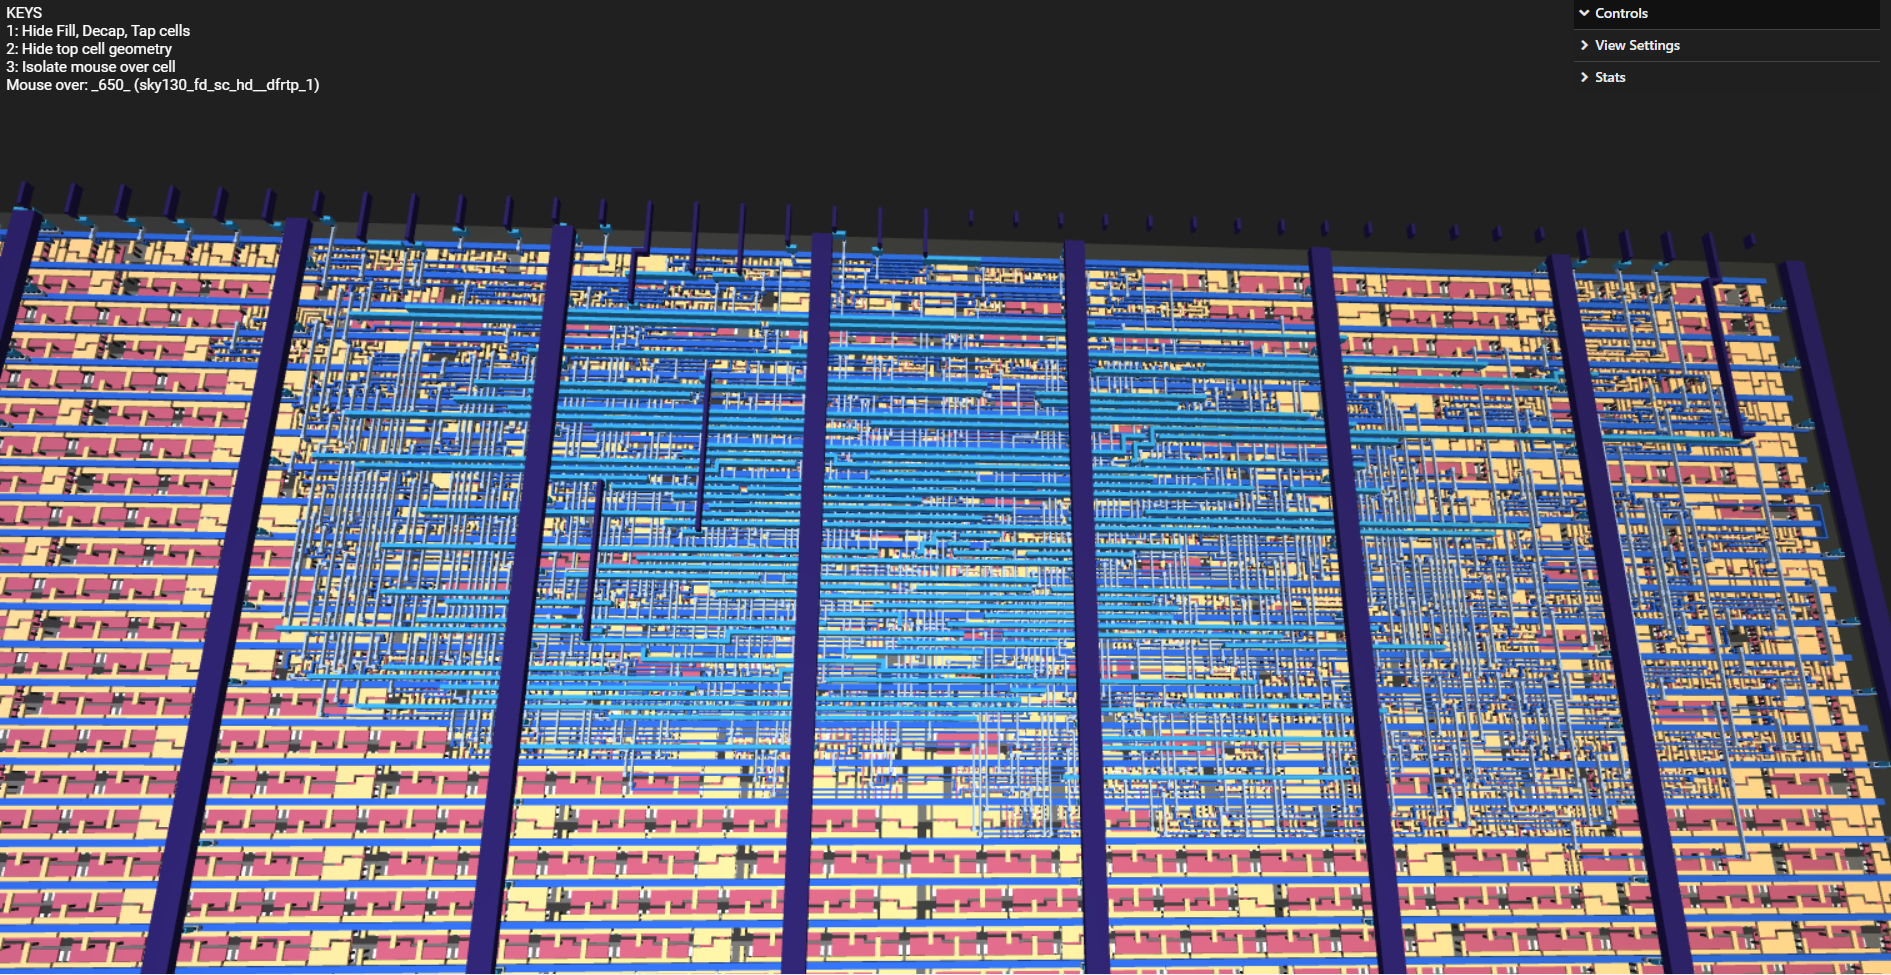
\includegraphics[width=\linewidth]{Pictures/Result_ASCII_3D_View.png}
        \caption{View 3D}\label{fig:ASCII_3D}
    \end{subfigure}
    \caption{ASCII text printer circuit layout}\label{fig:ASCII_Layout}
\end{figure}

\begin{figure}[H]
    \centering
    \begin{subfigure}[b]{0.45\textwidth}
        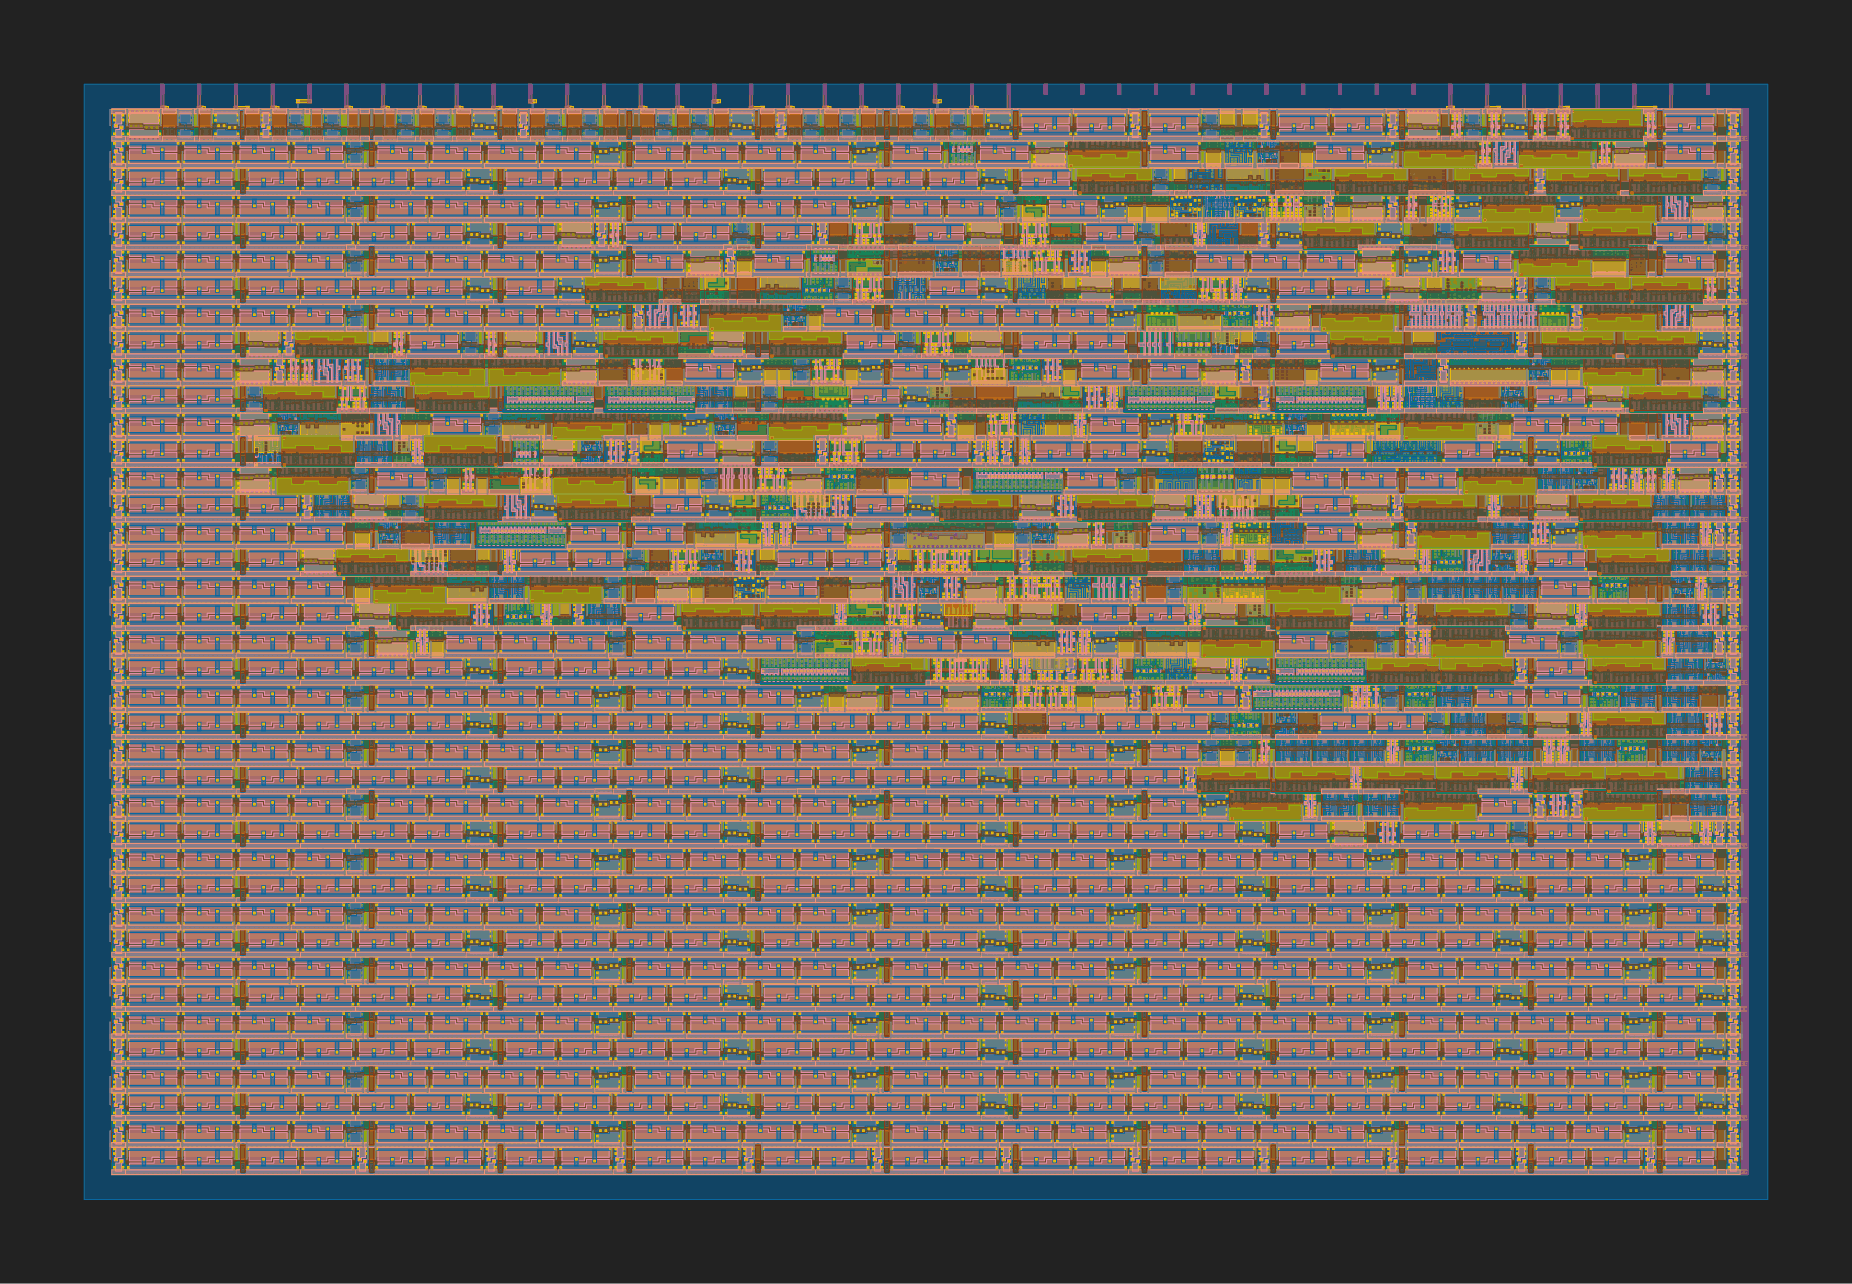
\includegraphics[width=\linewidth]{Pictures/Result_Pong_2D_View.png}
        \caption{View 2D}\label{fig:pong_2D}
    \end{subfigure}
    \begin{subfigure}[b]{0.45\textwidth}
        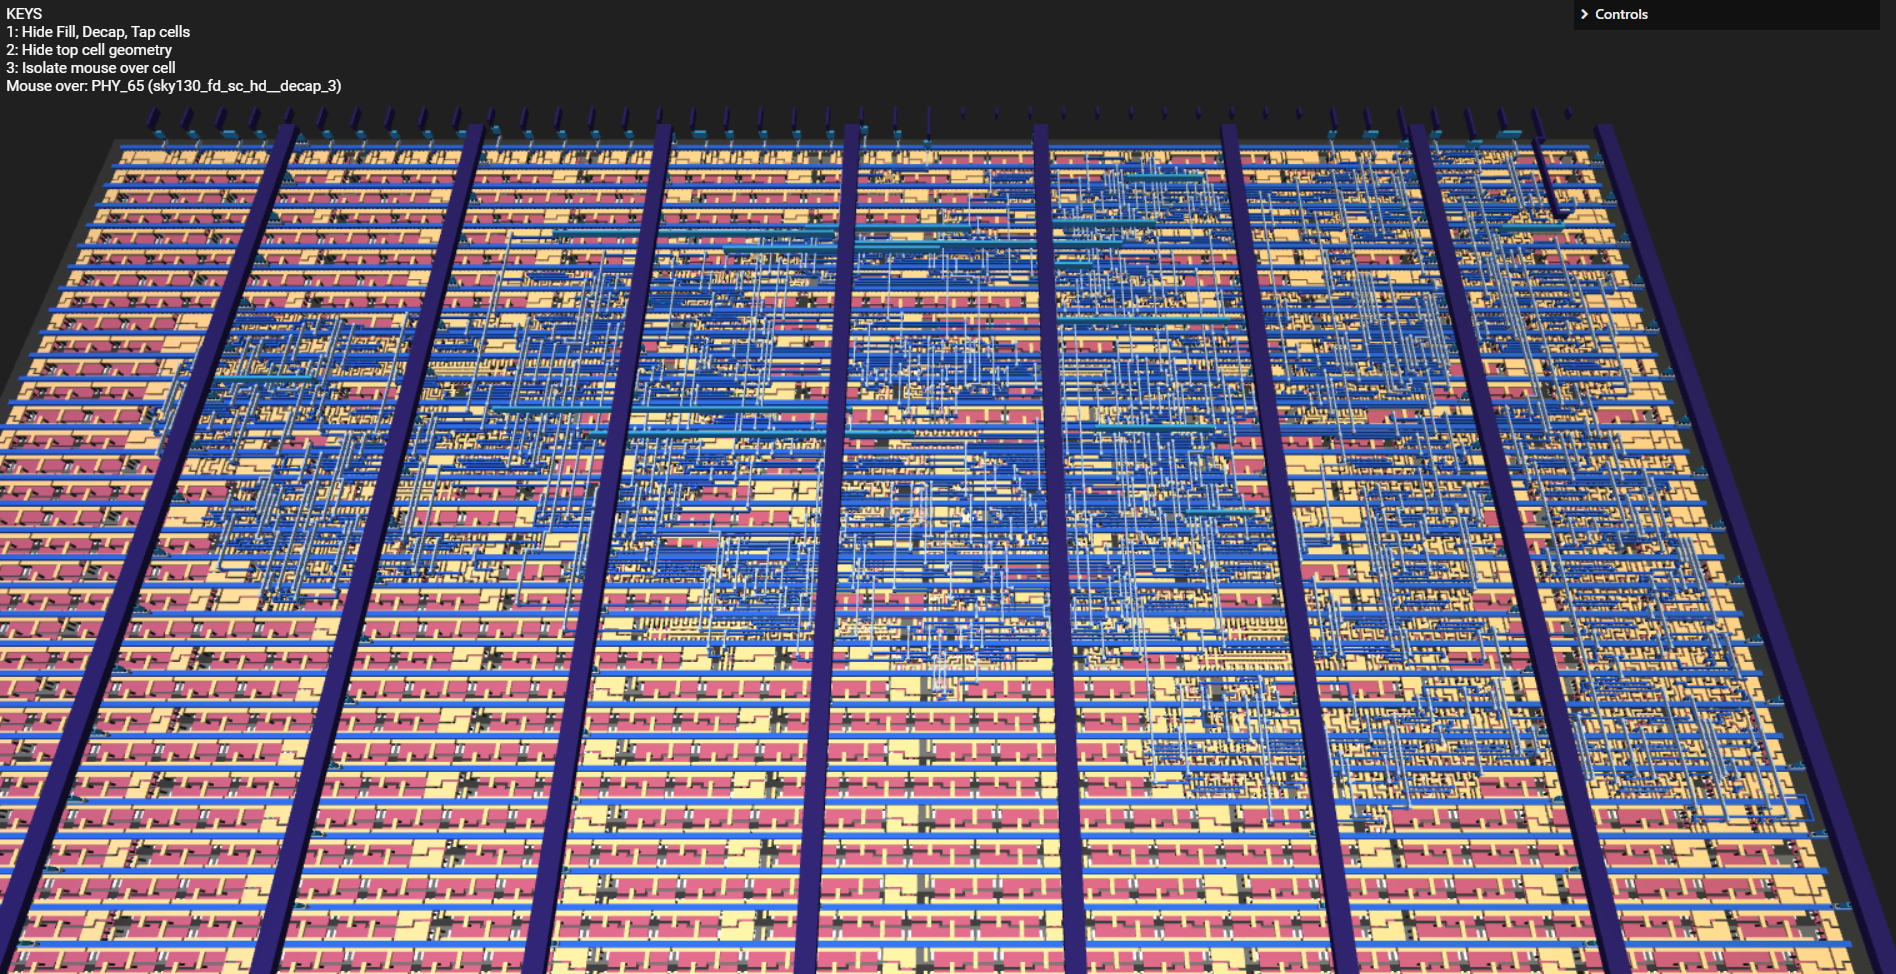
\includegraphics[width=\linewidth]{Pictures/Result_Pong_3D_View.png}
        \caption{View 3D}\label{fig:pong_3D}
    \end{subfigure}
    \caption{The Pong game layout}\label{fig:Pong_Layout}
\end{figure}

\begin{figure}[H]
    \centering
    \begin{subfigure}[b]{0.45\textwidth}
        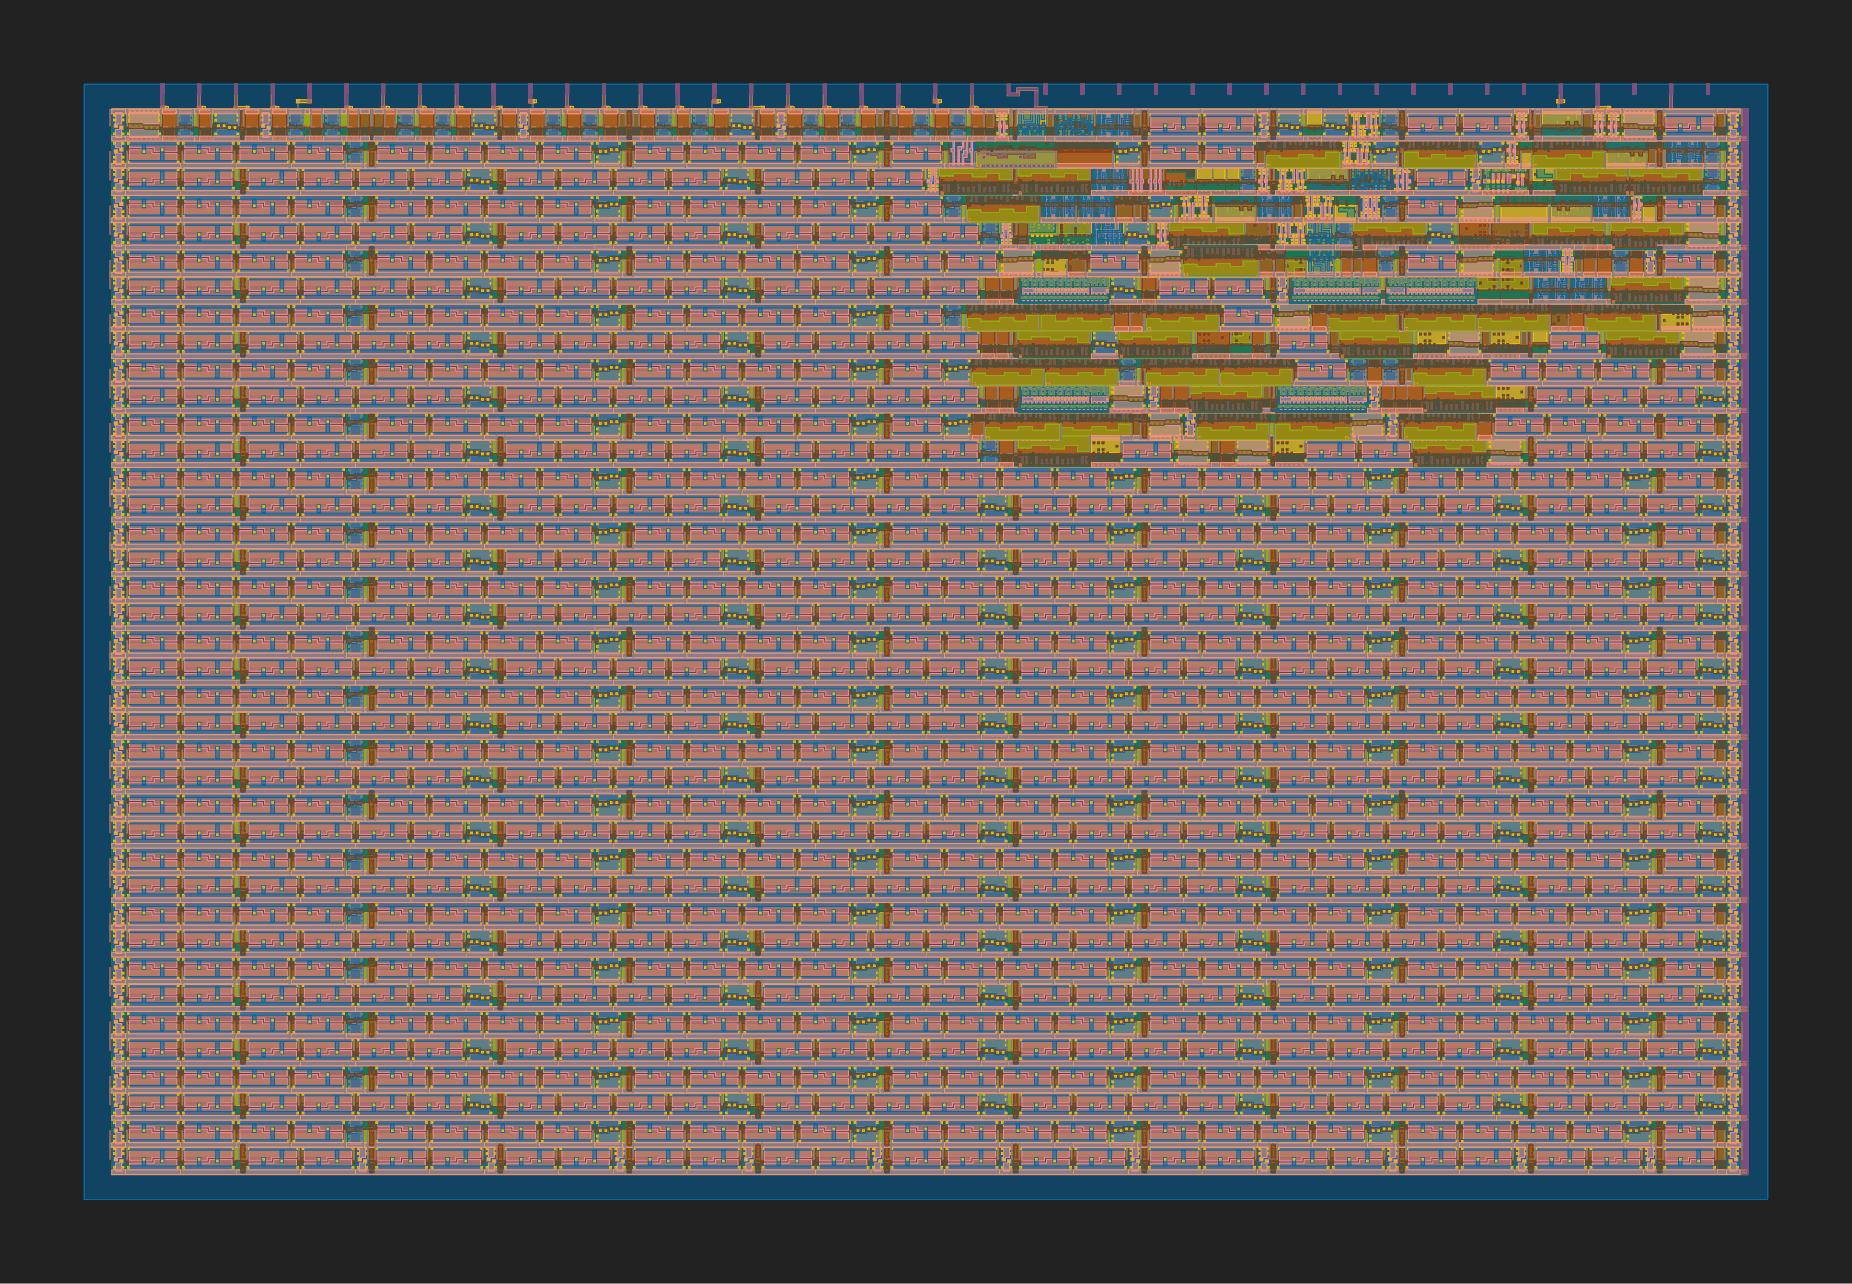
\includegraphics[width=\linewidth]{Pictures/Result_PWM_2D_View.png}
        \caption{View 2D}\label{fig:PWM_2D}
    \end{subfigure}
    \begin{subfigure}[b]{0.45\textwidth}
        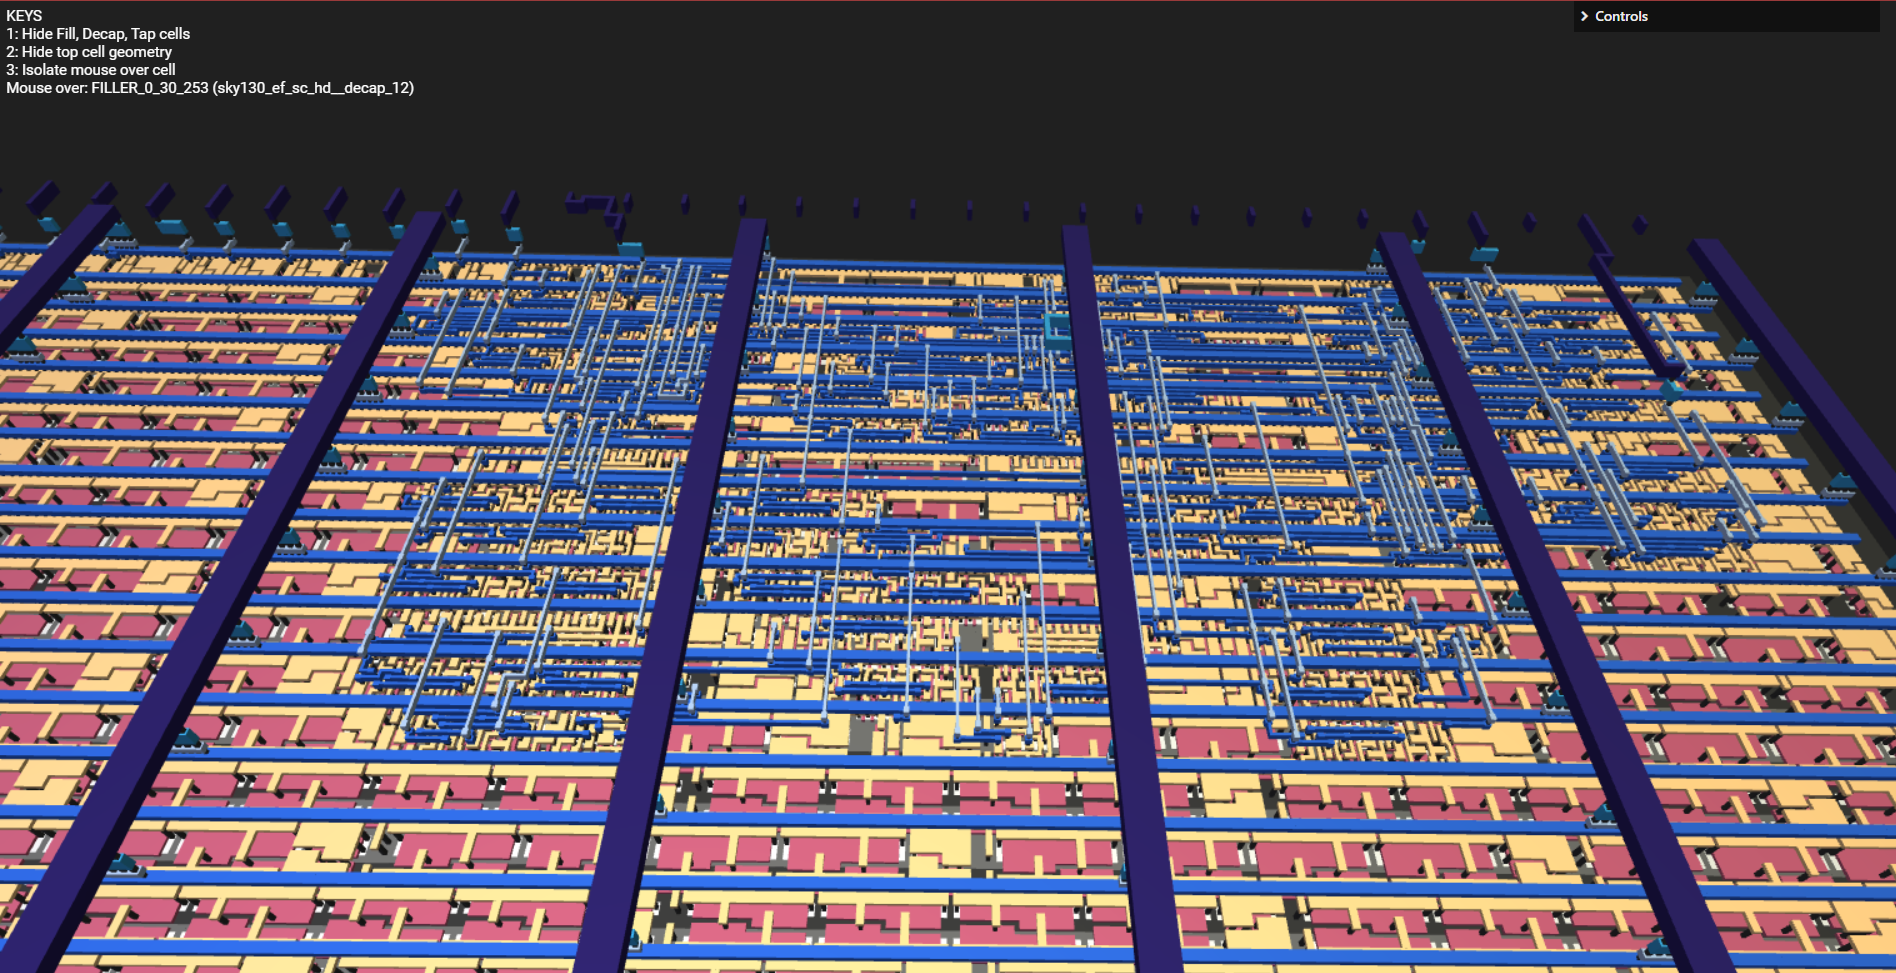
\includegraphics[width=\linewidth]{Pictures/Result_PWM_3D_View.png}
        \caption{View 3D}\label{fig:PWM_3D}
    \end{subfigure}
    \caption{Pulse Width Modulation generator layout}\label{fig:PWM}
\end{figure}

% Please add the following required packages to your document preamble:
% \usepackage{graphicx}


For a more in deep illustration on the complexity of the designs, figure \ref*{fig:Specific_Layout} 
has been included to showcase the different layers of the Pulse Width Modulation generator design.
The grey rectangles that can be observed in the figure are the N-wells for the transistors, 
the diffusion junction are the white rectangles, the pink rectangles are the polysilicon layers, 
the blue rectangles are the interconnect. 

 
\begin{figure}[H]
    \centering
        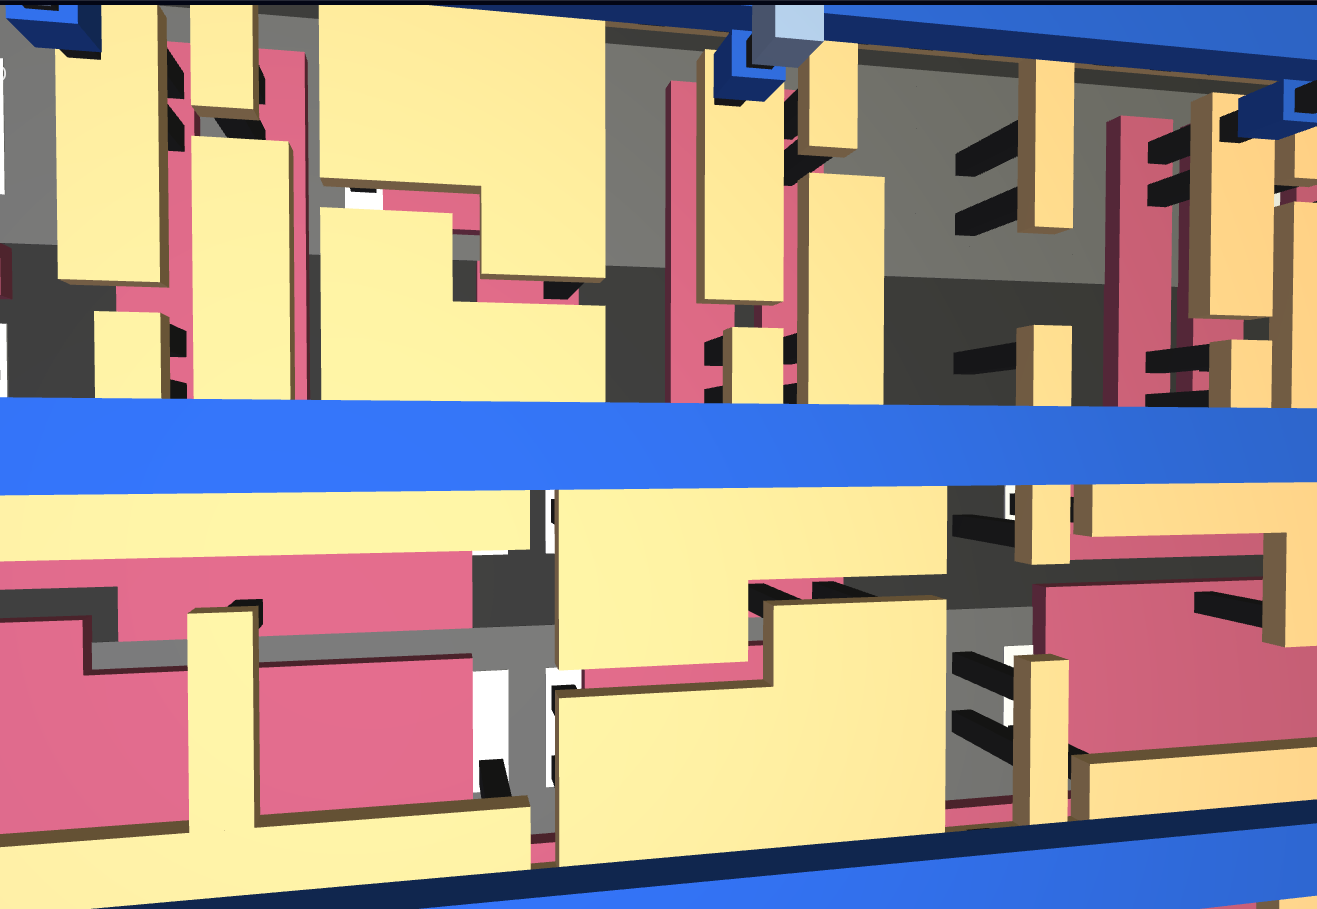
\includegraphics[width=\linewidth]{Pictures/Specific_Layout.png}
    \caption{Pulse Width Modulation generator layout}\label{fig:Specific_Layout}
\end{figure}

The Tiny Tapeout initiative has some limitations that are given by the nature of the project, one of 
the most important limitations to take inconsideration is the size of the die that each of the participants has 
to work with, due to this initiative being a multi-project wafer the size of the die is limited to 160um x 100um. 
This sizes may vary depending on the year of the initiative, due to how many projects are being submitted for fabrication. 
Table \ref*{tab:PorcentUtil} shows the percentage of the die that was utilized by each of the designs submitted.

\begin{table}[H]
    \centering
    \resizebox{\columnwidth}{!}{%
    \begin{tabular}{cc}
    \hline
    Circuit                                 & Porcentage utilize(\%) \\ \hline
    Multy stage path for delay measurements & 0.63                  \\
    ASCII Text Printer Circuit              & 17.87                 \\
    Implementation of the Pong game         & 28.82                 \\
    Pulse Width Modulation Generator        & 9.59                  \\ \hline
    \end{tabular}%
    }
    \caption{Porcentaje utilize in length of waver per circuit}\label{tab:PorcentUtil}
\end{table}


\begin{figure}
    \centering
    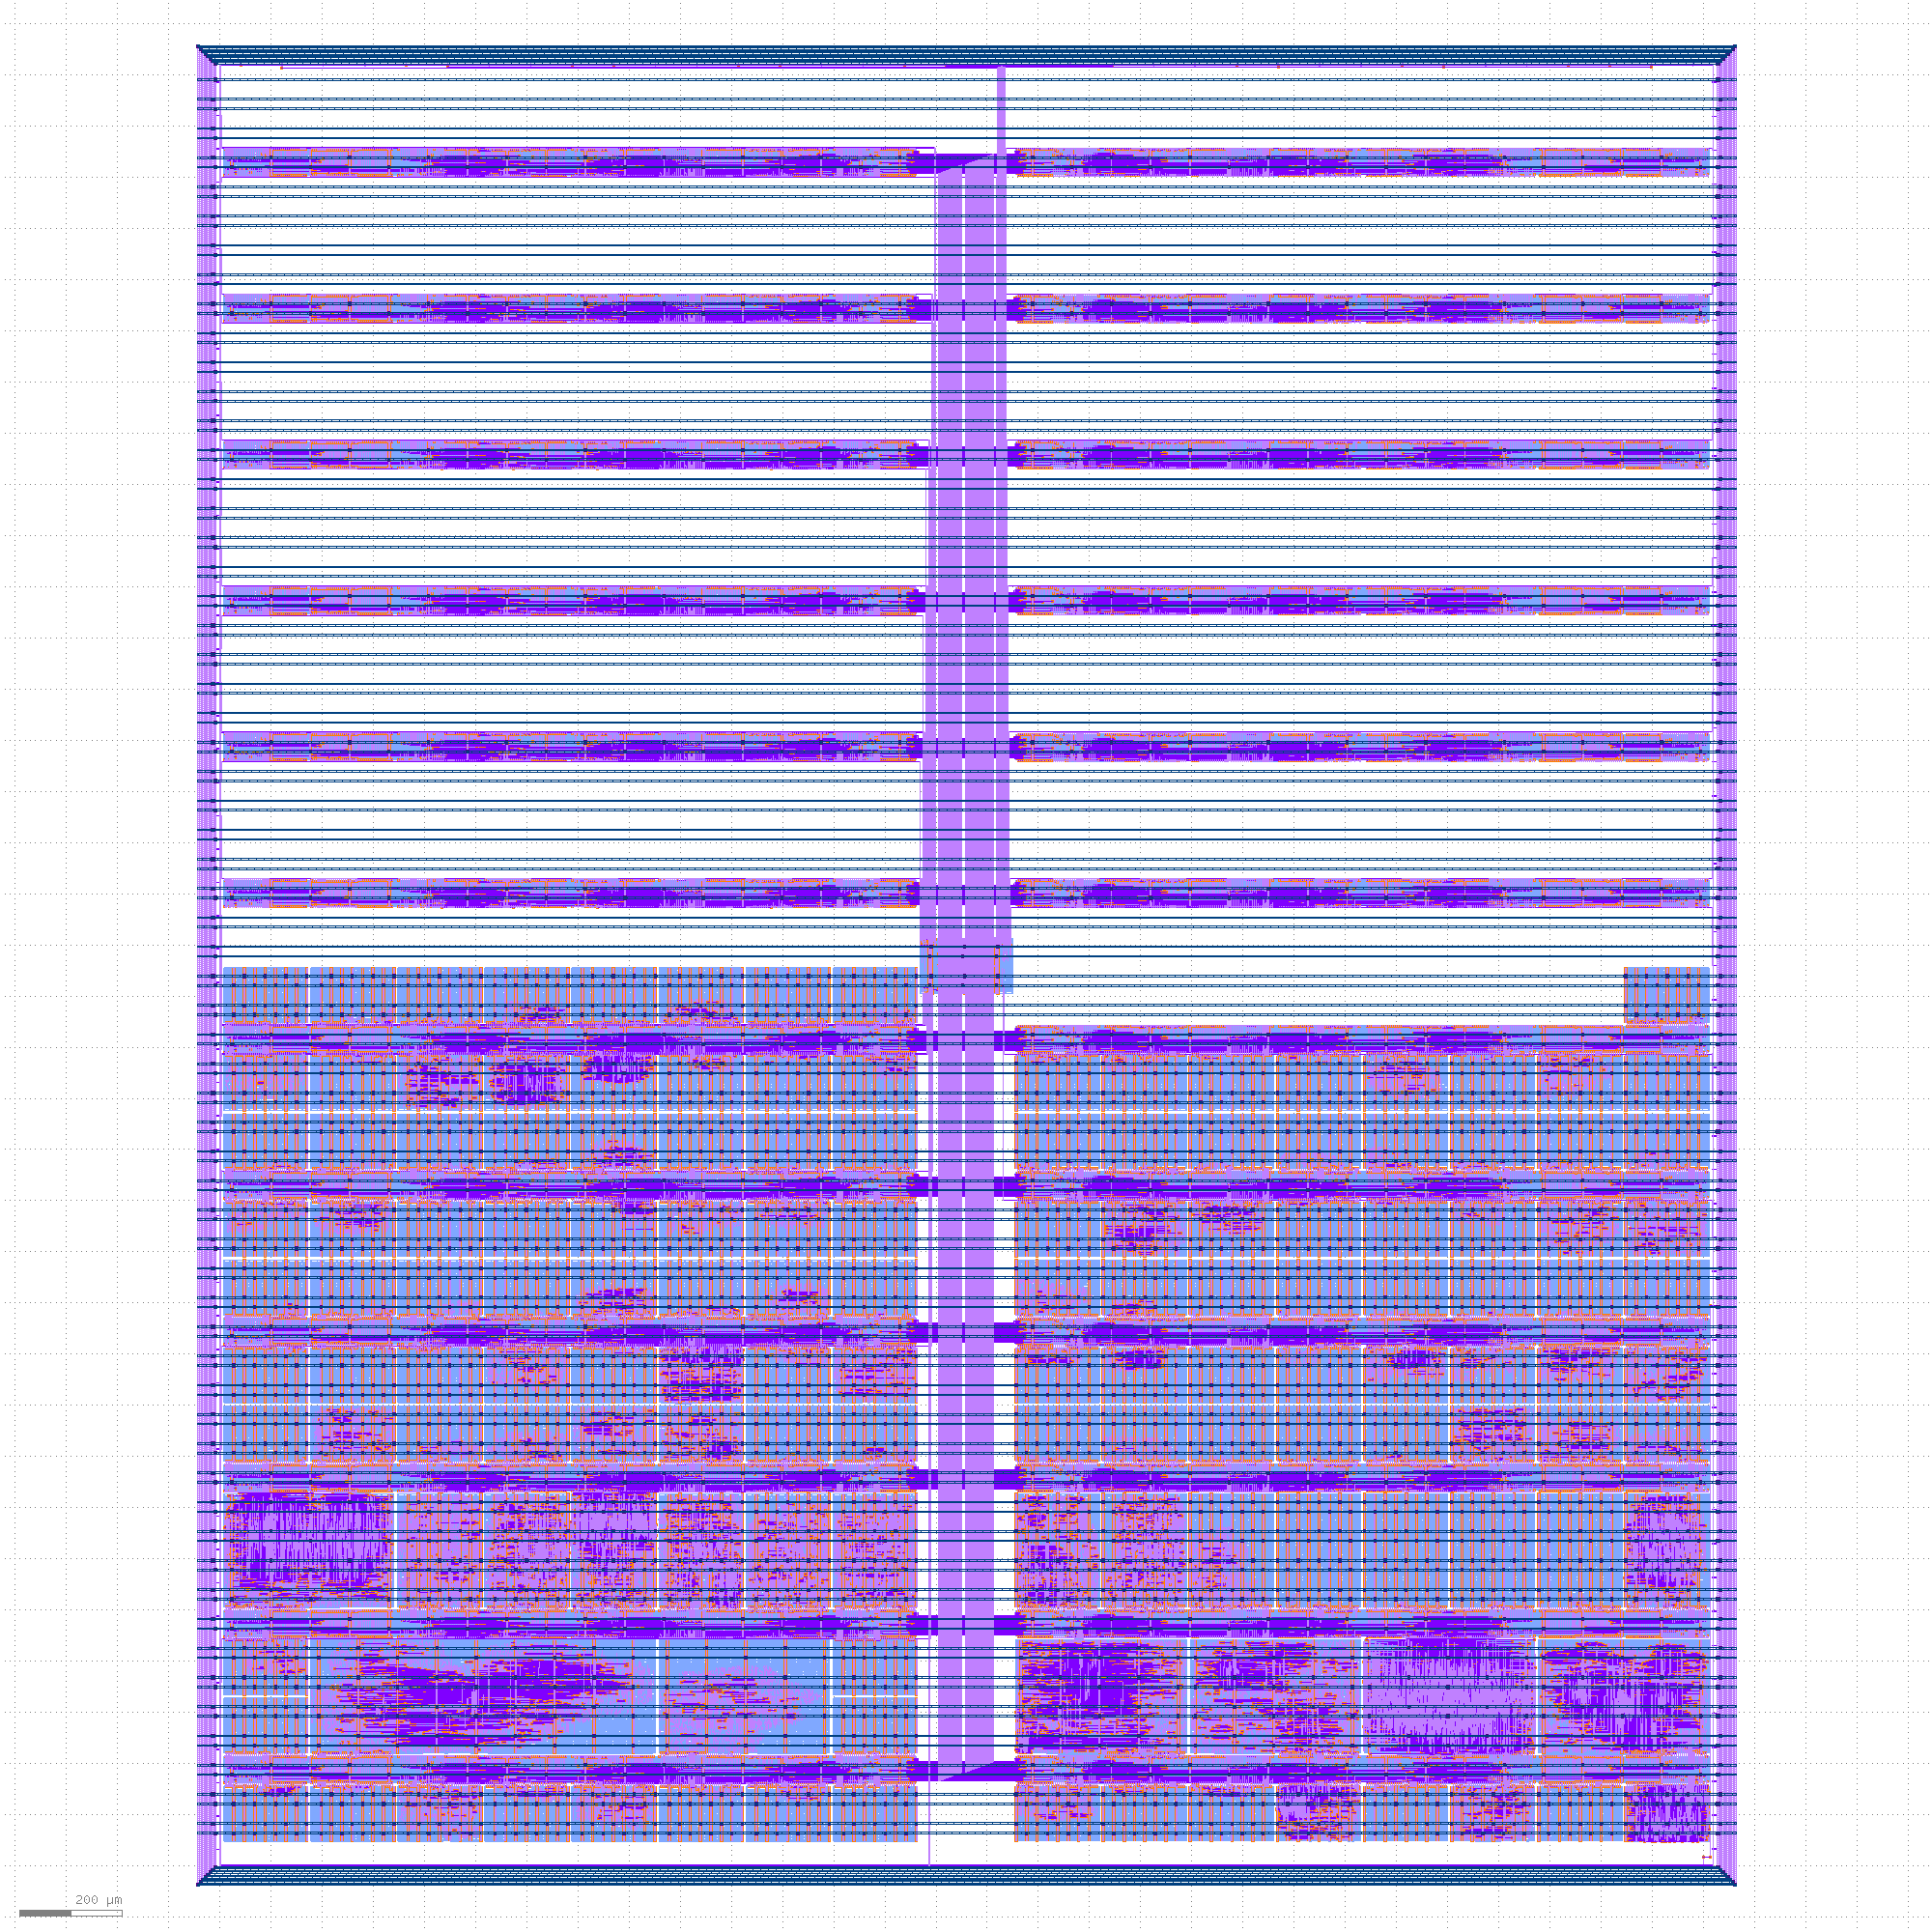
\includegraphics[width=\linewidth]{Pictures/fullfabricationdie.png}
    \caption{Full render of the die with 143 project}\label{fig:Layout}
\end{figure}


\section{Conclusion}
% Generate conclusions
\begin{enumerate}
    \item Four designs were created and submitted for manufacturing, encompassing a multistage path for delay measurement, an ASCII text printer circuit, the implementation of the Pong game, and a pulse width modulation generator.
    \item The four designs were submitted on the September 5th 2023 and were approved for manufacturing on October 10th 2023.
    \item Supporting materials, including videos and documentation, have been developed to facilitate the replication of the process by students.
    \item The Tiny Tapeout initiative has been successfully proven to be a viable option for educational purposes.
\end{enumerate}

\appendices
\section{Proof of the First Zonklar Equation}
Appendix one text goes here.

\section{}
Appendix two text goes here.


% use section* for acknowledgment
\section*{Acknowledgment}


The authors would like to thank...


% Can use something like this to put references on a page
% by themselves when using endfloat and the captionsoff option.
\ifCLASSOPTIONcaptionsoff
  \newpage
\fi

\begin{thebibliography}{1}

\bibitem{IEEEhowto:kopka}
H.~Kopka and P.~W. Daly, \emph{A Guide to \LaTeX}, 3rd~ed.\hskip 1em plus
  0.5em minus 0.4em\relax Harlow, England: Addison-Wesley, 1999.

\end{thebibliography}

% biography section
% 
% If you have an EPS/PDF photo (graphicx package needed) extra braces are
% needed around the contents of the optional argument to biography to prevent
% the LaTeX parser from getting confused when it sees the complicated
% \includegraphics command within an optional argument. (You could create
% your own custom macro containing the \includegraphics command to make things
% simpler here.)
%\begin{IEEEbiography}[{\includegraphics[width=1in,height=1.25in,clip,keepaspectratio]{mshell}}]{Michael Shell}
% or if you just want to reserve a space for a photo:

\begin{IEEEbiography}{Michael Shell}
Biography text here.
\end{IEEEbiography}

% if you will not have a photo at all:
\begin{IEEEbiographynophoto}{John Doe}
Biography text here.
\end{IEEEbiographynophoto}



\begin{IEEEbiographynophoto}{Jane Doe}
Biography text here.
\end{IEEEbiographynophoto}

% that's all folks
\end{document}


